\chapter{Styling}
\label{sec:styling}
% Old Ch. 6

We will demonstrate some styling techniques, by using an example we set up earlier on an abouts page (\cref{fig:aboutspage}). We have set up the contents of the abouts page in \cref{sec:pug1}, and now let's make it look prettier!
\vspace{6mm}

Less is used in place of CSS for reasons that we may explore down the chapter. But for now, we can just treat it as CSS. Because Less is a superset of CSS (i.e. all valid CSS codes are valid less codes). All knowledge you have learnt about CSS before can be transferable to Less, but we will start from scratch anyways for those of you who have not learnt CSS before.

% Less is used in place of CSS, to provide syntactic sugars\footnote{"Syntactic sugar" is a term for syntax changes in computer programming which make it easier for humans to code.} for us to make our lives easier, including nested styles and variables. 

\section{Logistics}

\subsection*{Where to write my code?}

As discussed in \cref{sec:lesslayout}, write your less code inside \texttt{app/styles/site}. 
\vspace{6mm}

Different from \cref{sec:classesids} where we write all our styling code in \texttt{layout.less} for simplicity. We should reorganise it so that \texttt{layout.less} should contain styles that is used in all/ multiple pages; \texttt{variables.less} should contain all variables; and other files should contain styles that is only used in the page with the same name as the style file.

When you create a new less file, remember to include it inside \texttt{site.less}

\begin{lstlisting}
// app/styles/site.less
@import "site/variables.less";

// Add your own site style includes here
@import "site/layout.less";
@import "site/index.less";
@import "site/abouts.less"; //we are styling the abouts page now
\end{lstlisting}

\subsection*{Syntax}

We actually have done some styling already in \cref{sec:classesids}. Refer to that section if you want a recap.
Let's now look at the same example again and we talk more about it.

\begin{lstlisting}[language=pug]
h2{
    color: red;
    margin: 4rem 0 4rem 0;
}
\end{lstlisting}

The HTML tag(s), class(es), or ID(s) before the curly braces is/are the elements you want to style. (more in \cref{sec:nestedstyles}) For now, we can just put one item there and there will be no confusion.
\vspace{6mm}

Then, what's inside the curly braces are the styles that we want to apply to the concerned elements. Each style consists of a \textbf{property} or \texttt{keyword} - \texttt{color} in our example, and \textbf{value(s)} - \texttt{red} in our example. When your property needs multiple values, separate them with a space, like what I did with the \texttt{margin} property, which as you will know later, needs 4 values. The property and the value(s) are separated by a colon. All styles are followed by a semi-colon. You can have multiple styles inside the curly braces. 
\vspace{6mm}

\subsection*{Further Resources}

I didn't have this piece of notes back when I first learned Less. Here is \href{https://youtu.be/YD91G8DdUsw}{the video}\footnote{Link: \url{https://youtu.be/YD91G8DdUsw}} that I used to learn the basics. 

CSS is well documented online, You could refer to the \href{https://www.w3schools.com/cssref/}{w3schools documentation}\footnote{Link: \url{https://www.w3schools.com/cssref/}} to learn how to use some more styling properties. 
However, there is no need to understand every CSS style, the common ones are listed below, and you can google search for the uncommon ones. :)

Moreover, the focus is on your ability to \textbf{combine different styling properties} to achieve what you want, not only on individual style properties. In that case, Google search serves you well. 

\section{CSS Properties}

\begin{table}[H]
    \centering
    \caption{Table of common Less (a.k.a. CSS) styling properties}
    \vspace{6mm}
    \begin{tabular}{|m{6.5em}|m{5em}|m{5.5em}|m{16em}|}
        \hline
        \textbf{Property} & 
        Options/ Examples & 
        Default &
        Description
        \\ \hline \hline
        
        \texttt{color}\tablefootnote{Sorry it has to be American spelling :(} &
        See \cref{sec:colours} & 
        \texttt{black} &
        Sets the colour of the text. 
        \\ \hline
        
        \texttt{background- color} &
        See \cref{sec:colours} &
        \texttt{transpar- ent}& 
        Sets the colour of the background.
        \\ \hline
        
        \texttt{text-align} &
        \makecell[lb]{
            \texttt{left}, \\
            \texttt{center}\tablefootnote{Sorry it has to be American spelling :(},\\ \texttt{right}, \\ \texttt{justify} \\
        } & 
        \texttt{left} &
        Sets the alignment of text. Justify means space is added between words so that both edges of each line are aligned with both margins.\tablefootnote{Note that justify might not work too well especially on mobile phones where the screen is thin, use left instead if that is the case.}
        \\ \hline
        
        \texttt{font-size} &
        \makecell[lb]{
            in \texttt{rem} \\(\cref{sec:rem})
        } &
        \texttt{1 rem} &
        Sets the font size of text
        \\ \hline
        
        \texttt{height}/ \texttt{width}&
        \makecell[lb]{
            in \texttt{\%}, \\
            in \texttt{px} \\
            in \texttt{rem}
        } & 
        / &
        Sets the width/ height of a certain element, usually an image. (\cref{sec:grid})
        \\ \hline
        
        \texttt{display} &
        \makecell[lb]{
            \texttt{block}, \\
            \texttt{none} \\
            \texttt{flex}
        } & 
        \texttt{block} &
        \texttt{block} is the normal one. Use \texttt{none} to hide the element. \texttt{flex} is used only with \cref{sec:flexbox}.
        \\ \hline
        
        \texttt{margin} &
        4 arguments in \texttt{rem} & 
        \texttt{0 0 0 0} &
        Sets the margin (additional spaces between elements) of the element in the order of top, right, bottom, left. (\cref{sec:marginpadding})
        \\ \hline
        
        \texttt{padding} &
        4 arguments in \texttt{rem} & 
        \texttt{0 0 0 0} &
        Sets the padding (additional spaces between elements) of the element in the order of top, right, bottom, left.  (\cref{sec:marginpadding})
        \\ \hline
        
        \texttt{border} &
        3 arguments &
        / &
        Sets the border of the element. 3 arguments - thickness (in \texttt{px}), type (usually \texttt{solid}) and colour (\cref{sec:marginpadding})
        \\ \hline
        
        \multicolumn{3}{|l|}{\texttt{font-weight: bold;}} &
        Makes the text bold
        \\ \hline
        
        \multicolumn{3}{|l|}{\texttt{font-style: italic;}} &
        Makes the text italic
        \\ \hline
        
    \end{tabular}
\end{table}

I would like to stress that it is unnecessary to remember every CSS property by heart. For example, whenever I need to make some text italic, which is seldom the case, I would search "italic css" and \texttt{font-style: italic;} would pop up. 

\subsection{Colours}
\label{sec:colours}
The colour for properties like \texttt{color}, \texttt{background-color} and \texttt{border} can be specified in RGB colour codes, e.g. \texttt{\#FFFFFF} indicates white, \texttt{\#FF0000} indicates red. You do not need to dig deep on how the colour code works, you could just find your desired colour using a random RGB colour picker online, such as the one you get  \href{https://www.rapidtables.com/web/color/RGB_Color.html}{following this URL}\footnote{Choose your colour: \url{https://www.rapidtables.com/web/color/RGB_Color.html}}.   \href{https://www.w3.org/wiki/CSS/Properties/color/keywords}{Common colours}\footnote{Full list of "common" colours: \url{https://www.w3.org/wiki/CSS/Properties/color/keywords}} can be specified in text for your convenience, like \texttt{red}.

\begin{lstlisting}
.blue-text{
    color: #0000FF; 
}
\end{lstlisting}

The default value for \texttt{background-color} is \texttt{transparent}. It is important to distinguish between a white background and a transparent background. 

\subsection{Unit for size - \texttt{rem}}
\label{sec:rem}

The unit for size for properties like \texttt{font-size}, \texttt{margin} and \texttt{padding} is interesting. As \texttt{rem} scales based on screen size while other units like \texttt{px} will not, \texttt{rem} is the ideal unit for text, margins and paddings. \footnote{For more information, refer to \url{https://engageinteractive.co.uk/blog/em-vs-rem-vs-px} if interested.} Normal text should have a font size of 1 rem. Therefore, 1.25rem is used in my example in \cref{sec:classesids} to indicate a slightly larger text but not overwhelmingly large.

\begin{lstlisting}[language=pug]
// app/styles/site/abouts.less
.large-text{
    font-size: 1.25rem;
}
\end{lstlisting}

Size of images might be an exception, using \texttt{px} might be more convenient because you might not want your images to scale on screen size change, or more commonly, we will use the \texttt{width: 100\%} technique introduced in \cref{sec:width}.

\section{Browser developer tools} 

Tools provided by browsers can help significantly with styling. Every browser got their own one, accessible in sightly different ways and sightly different interfaces. I will be using Brave (similar to Google Chrome) in this piece of notes.

If you are using a different browser, or would like to know more details, refer to \href{https://www.hostinger.co.uk/tutorials/website/how-to-inspect-and-change-style-using-google-chrome}{this documentation}, with illustrations on how to open the developer tools for different browsers for your convenience.
\vspace{6mm}

First of all, open one of our HTML files in the \texttt{docs} folder. Then right click, then select \texttt{inspect}. Then a window should appear on the side, select the \texttt{Elements} menu and the \texttt{styles} menu. (see \cref{fig:devtools})

\begin{figure}[h]
\centering
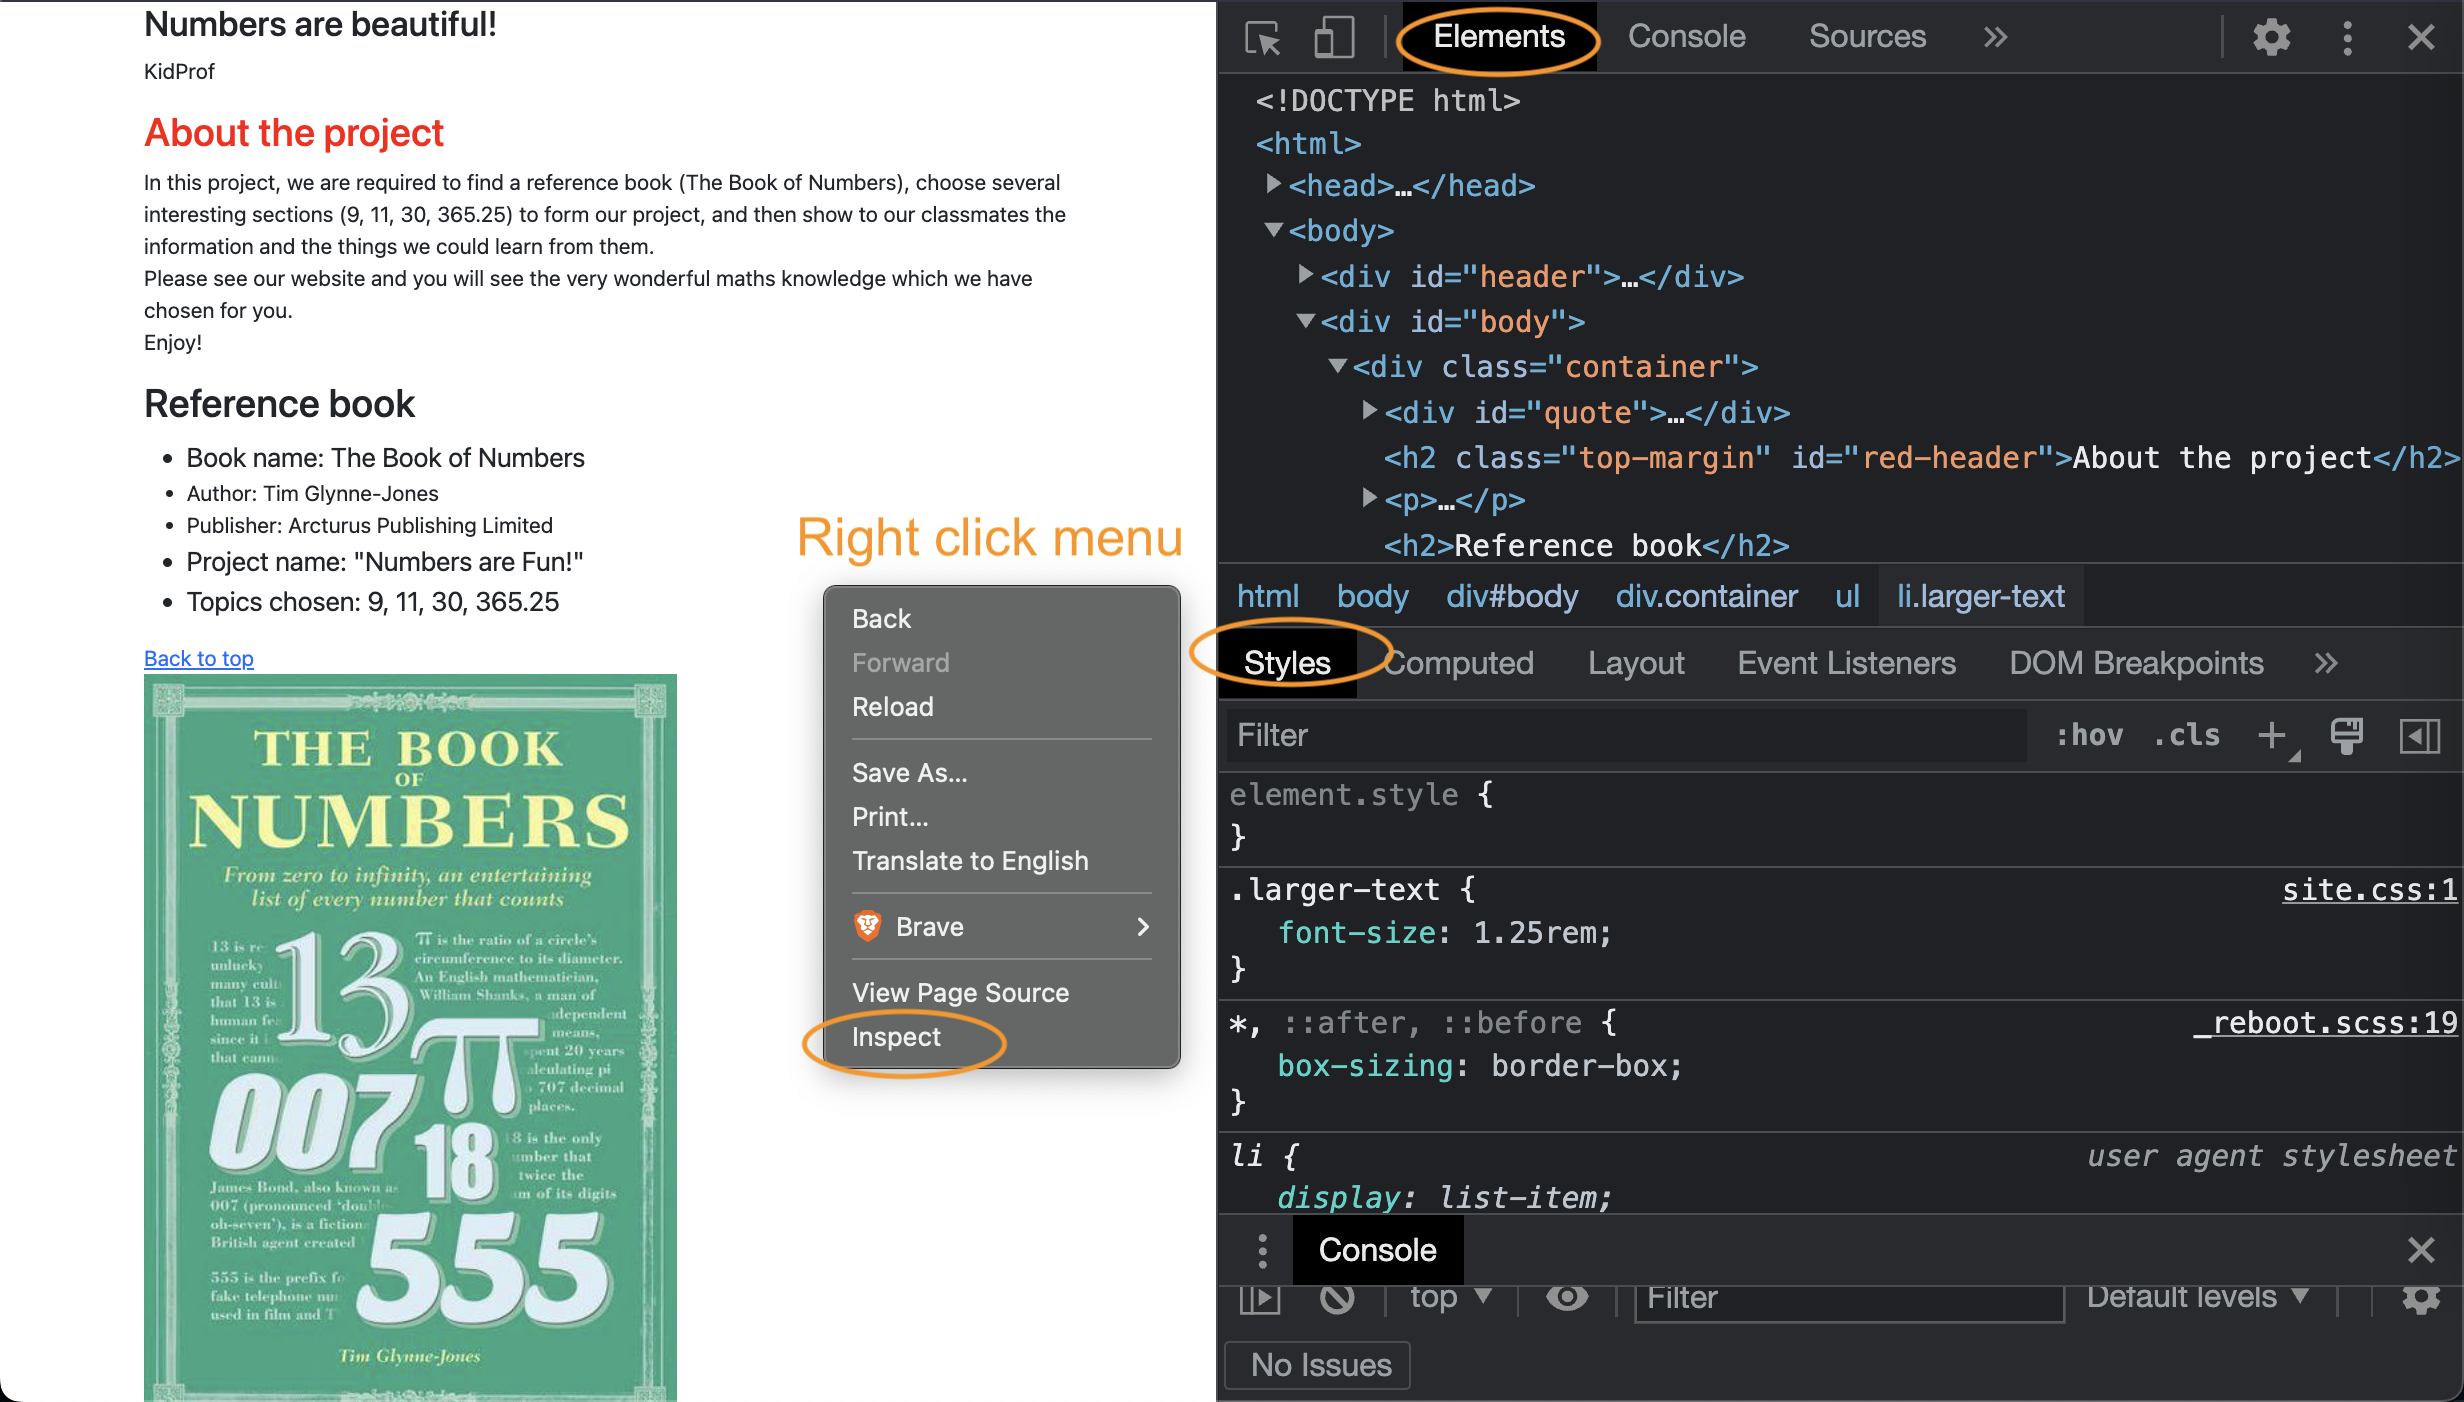
\includegraphics[width=14cm]{images/chn6-devtools.png}
\caption{The developer tools menu}
\label{fig:devtools}
\end{figure}

In the \texttt{Elements} menu, you can select an element that you are interested in, and you can see the styles applied to it in the \texttt{styles} menu. Alternatively, you can right click on that element and select \texttt{inspect} to focus on that element as well.
\vspace{6mm}

\begin{figure}[h]
\centering
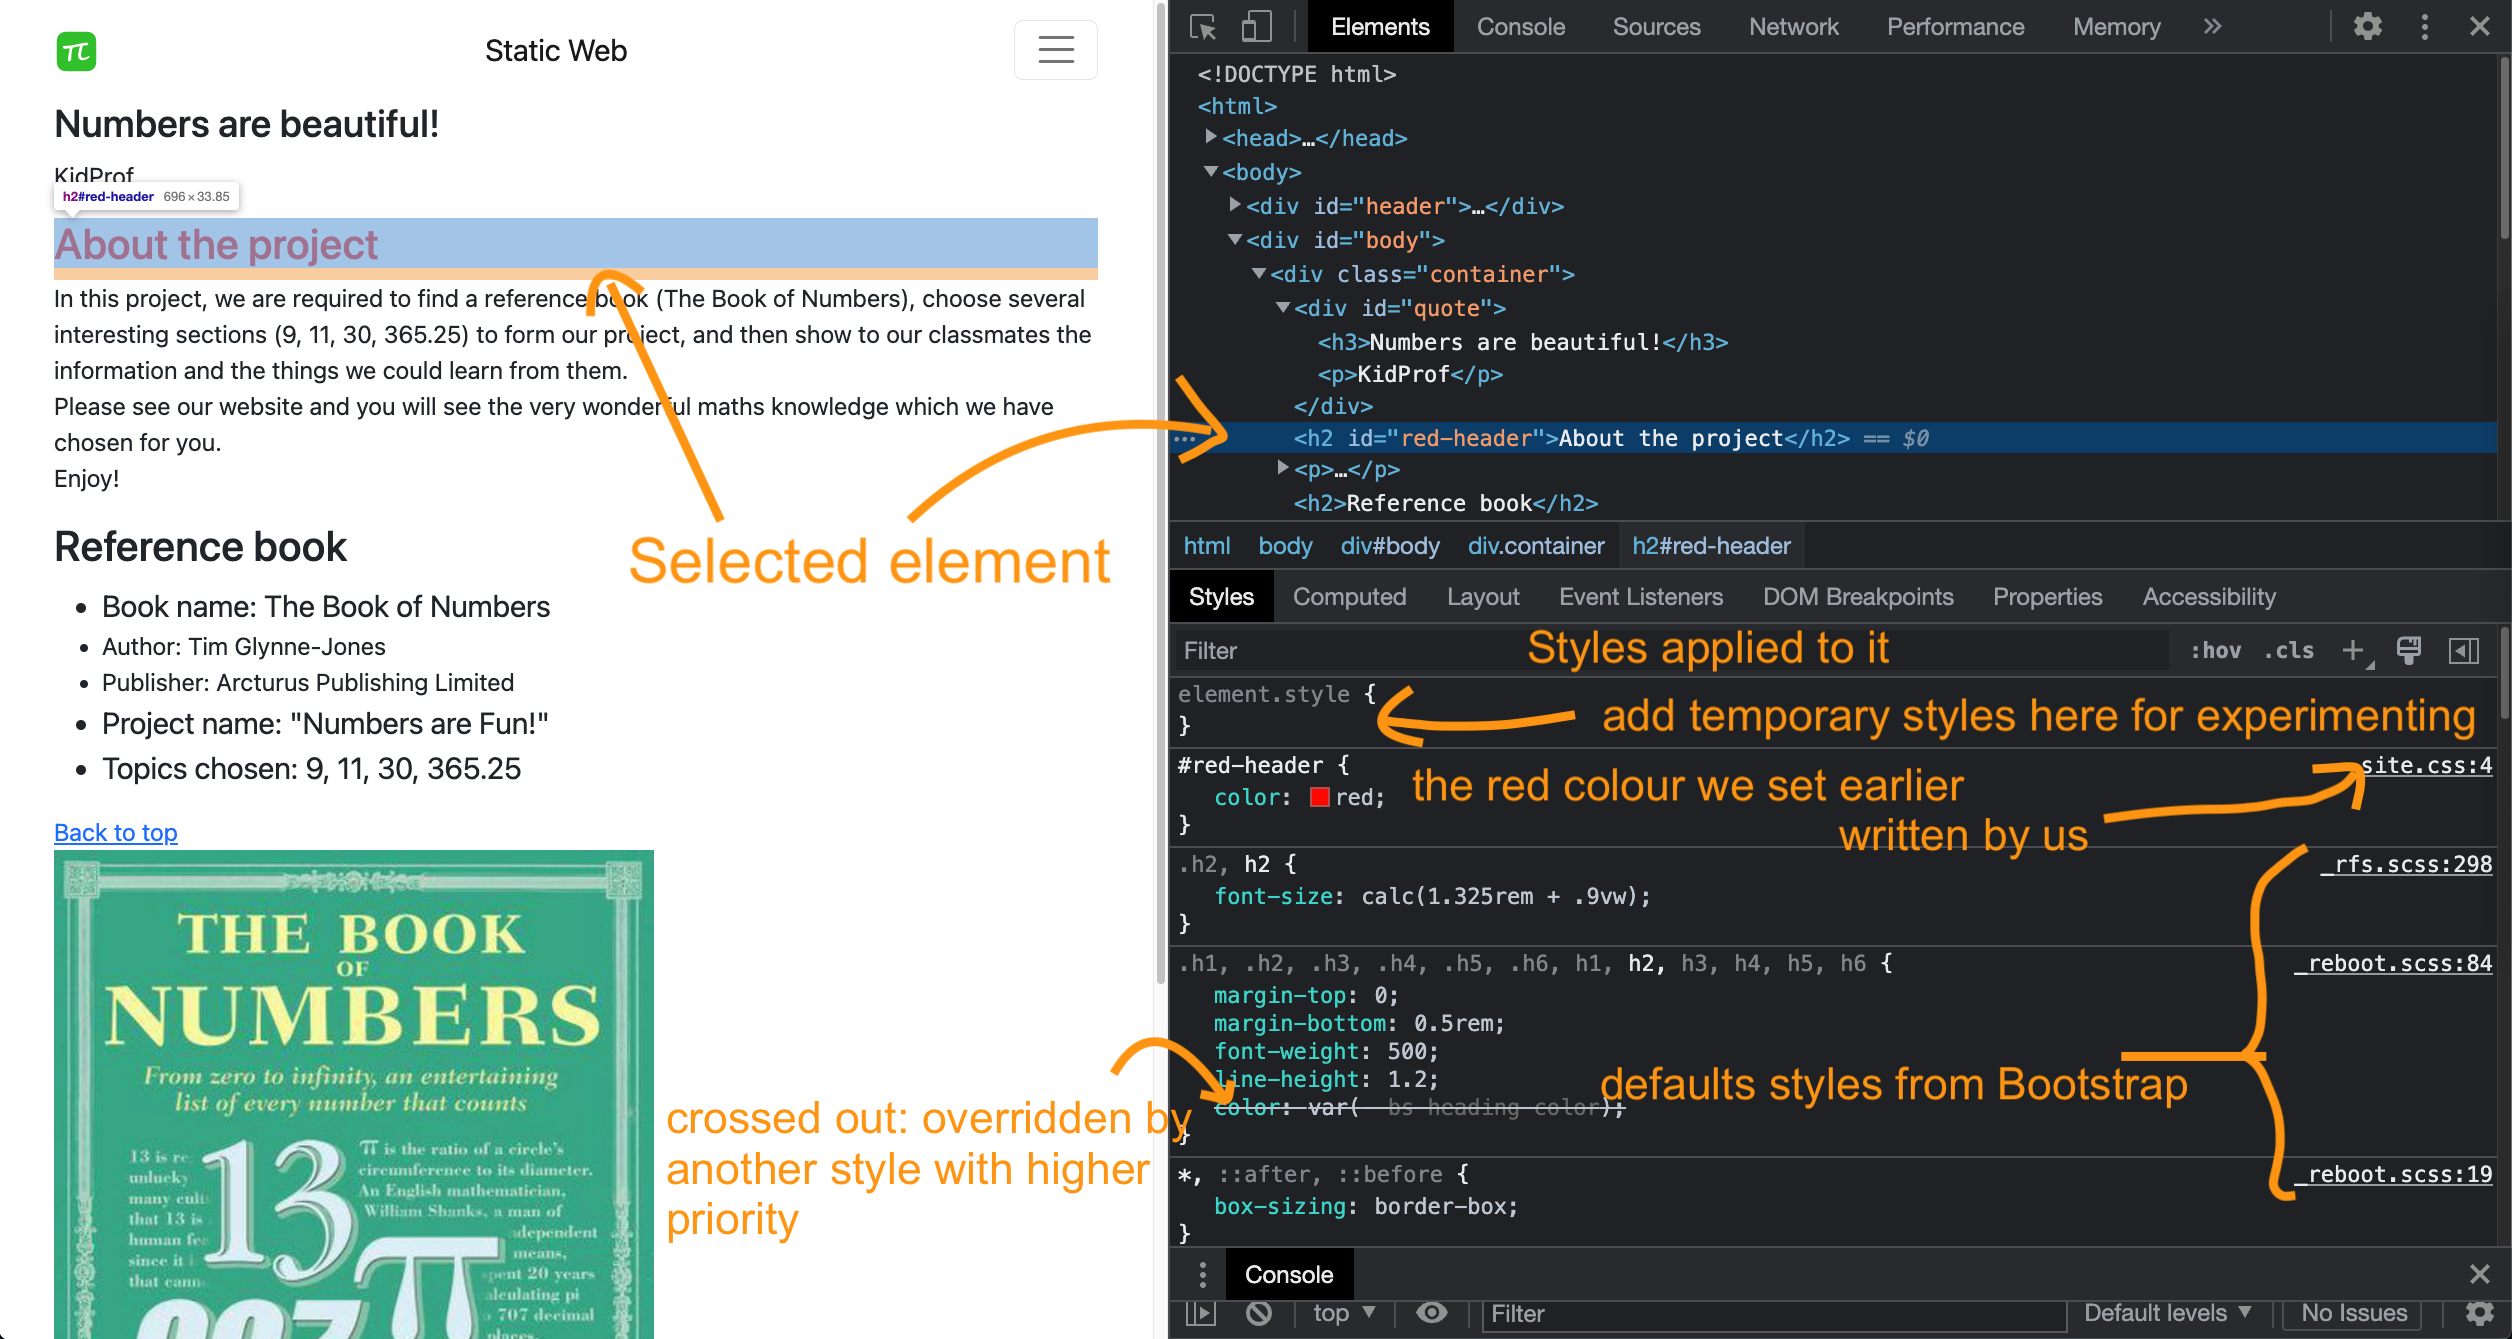
\includegraphics[width=14cm]{images/chn6-devtools2.png}
\caption{The developer tools menu, focusing on a specific element}
\label{fig:devtools2}
\end{figure}

We can write some temporary styles under \texttt{element.style} (as indicated in \cref{fig:devtools2}), the things we write there would be cleared when we refresh the page. It is a common practice to test out the styling properties that we want to apply to the element(s) here first, then we only copy our code to the less file when we are satisfied, this saves time building the code and defining classes and IDs. Again, be sure to record down what you styled before refreshing the page, as the styles will be gone on refresh. 
\vspace{6mm}

Remember we are planning to make our web page \textbf{responsive}, meaning that the elements should rearrange and scale, making out web page look good on mobile. To simulate what you will see on mobile devices, just enlarge the developer tools to the right to shrink the page, or you can use a mobile phone simulator by Chrome by clicking one of the buttons on the top left of the developer tools menu.

You will also notice in \cref{fig:devtools2} there is a crossed out style. It means the default black colour of the text is being overridden by our style that sets it to red. More explanation would be in \cref{sec:stylingpriority}.
\vspace{6mm}

\textbf{Remember to the browser styling tools often}

\section{Nested styles}
\label{sec:nestedstyles}

Things could get complicated when we try to reference more complex things from the Pug file.

There are three types of nesting. 

\begin{itemize}
\item \textbf{Within} - spaces in between

We are styling all \texttt{h3} within \texttt{\#quote} in the following example.
    
\begin{lstlisting}[language=pug]
// app/styles/site/abouts.less
#quote h3 {
    text-align: center;
}
\end{lstlisting}
    
\begin{lstlisting}[language=pug]
//- app/templates/views/abouts.pug
#quote 
    h3 Numbers are beautiful    <-- THIS ONE
    ...
h3 Will not be styled as it is outside #quote
\end{lstlisting}

Less allows we to also do the nesting like this, that is equivalent to \texttt{\#quote h3}. I need to stress that this is only valid in Less but not in normal CSS. (You can verify this by comparing our less code with \texttt{dist/styles/site.css})

\begin{lstlisting}[language=pug]
// app/styles/site/abouts.less
#quote {
    h3 {
        text-align: center;
    }
}
\end{lstlisting}

\item \textbf{and} - no spaces in between

We are styling all elements with BOTH classes \texttt{.beautiful} and \texttt{.cooler} in the following example.
    
\begin{lstlisting}[language=pug]
// LESS
.beautiful.cooler {
    font-style: italic;
}
\end{lstlisting}

\begin{lstlisting}[language=pug]
//- PUG
p.beautiful.cooler Will be styled    <-- THIS ONE
p.beautiful Will not be styled as it only has one class
.beautiful
    p.cooler Will not be styled, do not mix it up with the "within" case
\end{lstlisting}

\item \textbf{or} - comma in between

We are styling all elements with either classes \texttt{.beautiful} or \texttt{.cooler} in the following example.
    
\begin{lstlisting}[language=pug]
// LESS
.beautiful, .cooler {
    font-style: italic;
}
\end{lstlisting}

\begin{lstlisting}[language=pug]
//- PUG
p.beautiful.cooler Will be styled 
p.beautiful Will not be styled 
p.cooler Will be styled
\end{lstlisting}

\end{itemize}

(All elements in the above examples can be any tags, classes or IDs.)

As an example, let's style the quote in our abouts page example.

\begin{lstlisting}[language=pug]
//- templates/views/abouts.pug
#quote
    h3 Numbers are Beautiful
    p KidProf
\end{lstlisting}

First we add a grey \texttt{background-color} to the quote. We also want \textbf{all} the text within it to be white. At the same time, I want \textbf{only} the \texttt{h3} tag to be centred and white while \textbf{only} the \texttt{p} tag to be right aligned.

\begin{lstlisting}[language=pug]
// app/styles/site/abouts.less
#quote {
    background-color: #888;
    color: white;
    h3{
        text-align: center;
        font-style: italic;
    }
    p{
        text-align: right;
    }
}
\end{lstlisting}

\begin{figure}[h]
\centering

\includegraphics[width=15cm]{images/chn6-quote1.png}
\caption{Result of the quote up to \cref{sec:nestedstyles}}
\end{figure}


\section{Size and positioning}

In this section we will focus on getting the book of numbers image into position with the correct size in our sample abouts page as an example. 

First and foremost, we give the image an ID. 

\begin{lstlisting}
//- app/templates/views/abouts.pug
img#bookofnumbers(src="images/bookofnumbers.jpg")
\end{lstlisting}

\subsection{Width and height}
\label{sec:width}

We can set the size of the image by using \texttt{width} and \texttt{height}.

We can try either of these

\begin{itemize}
\item Only setting the width or height in px
    
\begin{lstlisting}[language=pug]
#bookofnumbers{
    width: 700px;
}
\end{lstlisting}

You can see it's height scales with the width, this is the behaviour when only \texttt{height} or \texttt{width} is specified.

However, there seems to be no number that does the job perfectly in our case. Making it too small will make the image too small for large screens, and making it too large makes the image too large to be shown in full on small screens. 

This approach sometimes works when the image is small, smaller than the width of small screens. (e.g. mobile phones)

\begin{figure}[h]
\centering
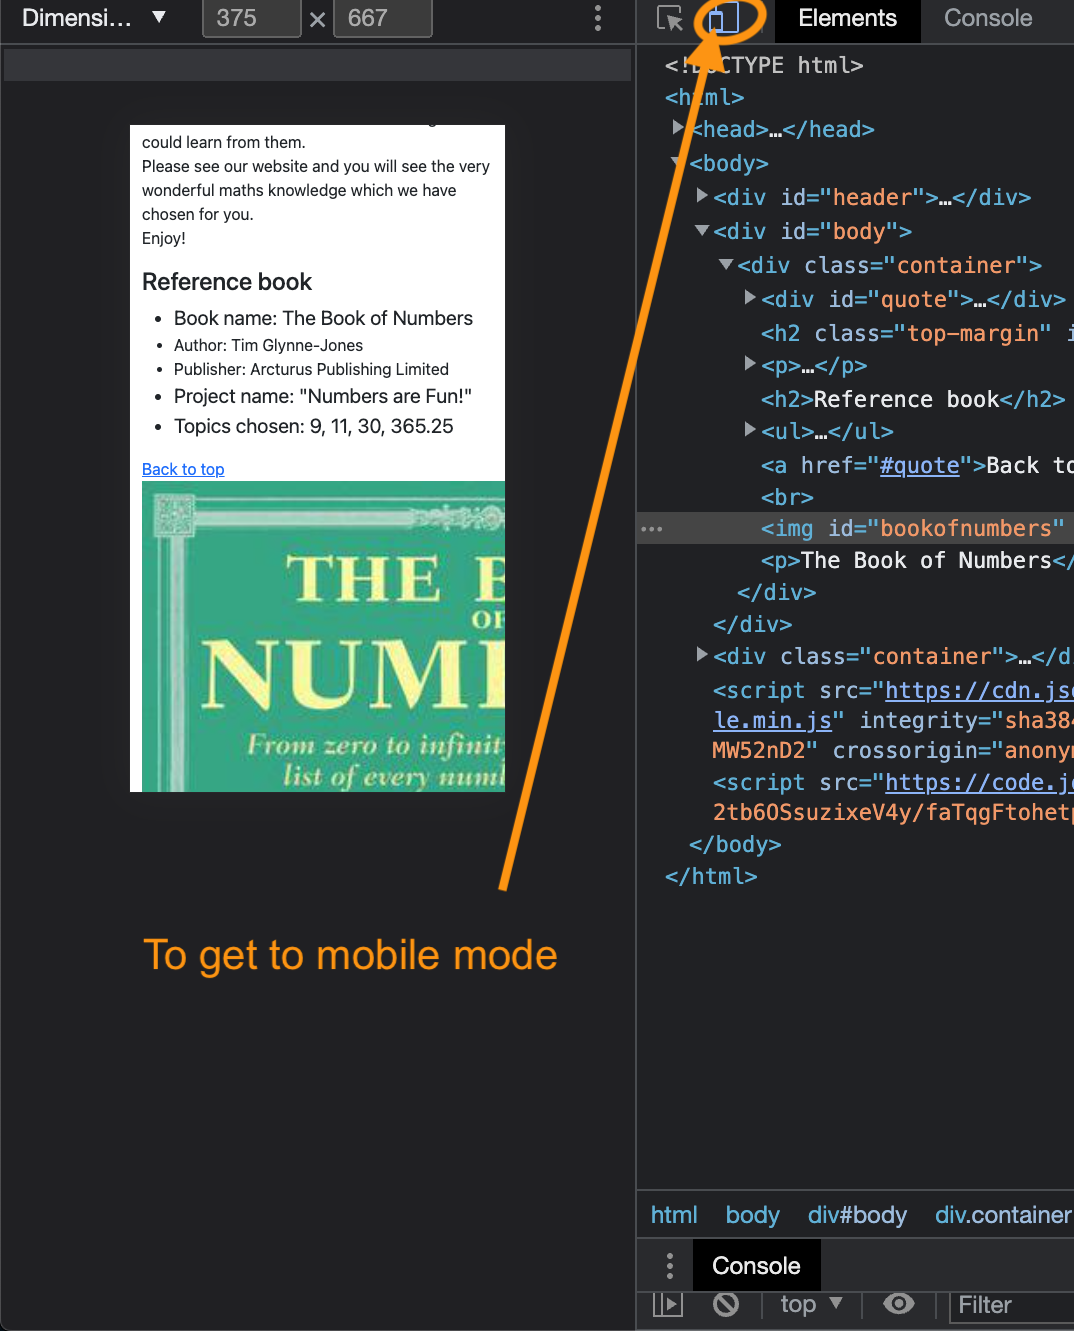
\includegraphics[width=7cm]{images/chn6-widthonly.png}
\caption{Result of setting width to 700px, looks bad on small screens (also shows you the button for the mobile view in the developer tools)}
\end{figure}

\item Setting both the width and height

\begin{lstlisting}[language=pug]
#bookofnumbers{
    width: 700px;
    height: 100px;
}
\end{lstlisting}

The image scales according to the width and height you specified, the aspect ratio changes as well. It usually comes out to be quite ugly as the aspect ratio is distorted. If you find yourself calculating the aspect ratio by hand before entering it, you probably don't need to because you can use the previous approach (providing either width or height) and the image will then be scaled based on its aspect ratio.

This approach usually gives ugly results and is seldom used.

\begin{figure}[h]
\centering

\includegraphics[width=10cm]{images/chn6-widthandheight.png}
\caption{Result of setting both width and height, would not recommend}
\end{figure}

\item Setting the width or height in percentages

\begin{lstlisting}[language=pug]
#bookofnumbers{
    width: 100%;
}
\end{lstlisting}

We are now setting the image to be as wide as it's parent, in this case it is the \texttt{.container} (see \cref{sec:container}), it will be aligned well with other texts. 

Again, there seems to be no number that fits perfectly. Setting it to 100\% makes the image super large for large screens, while setting it to a smaller number, like 50\%, makes the image too small in smaller screens.

\begin{figure}[h]
\centering
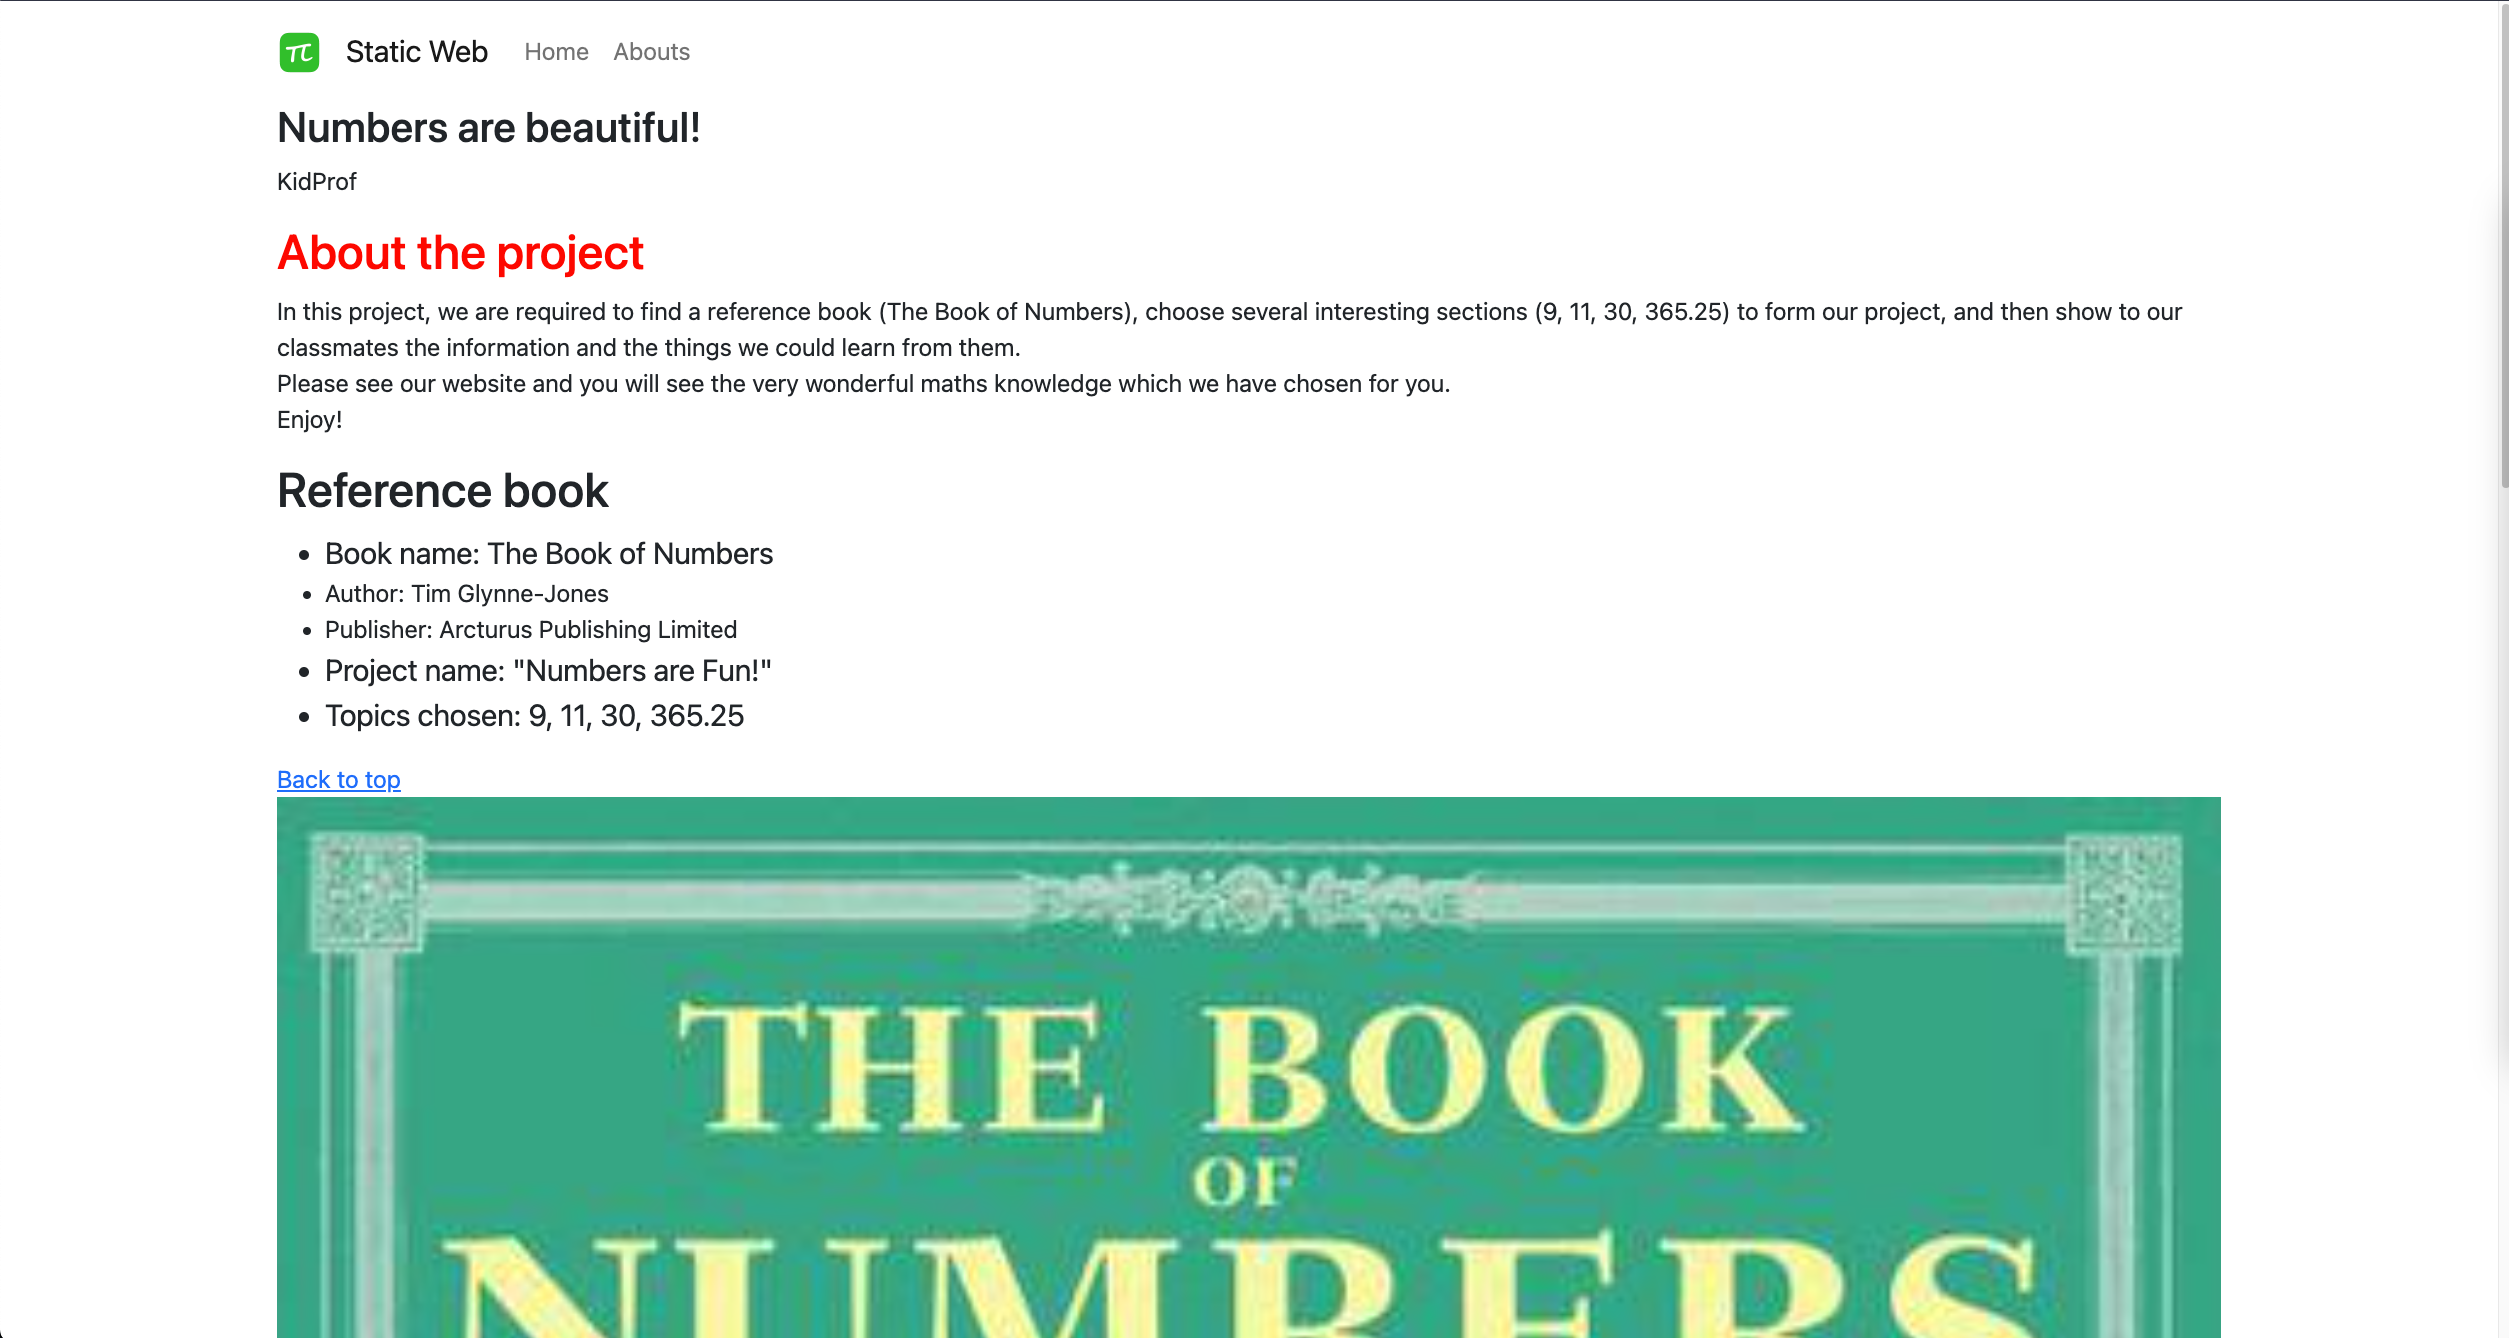
\includegraphics[width=15cm]{images/chn6-w100.png}
\caption{Result of setting width to 100\%, too big for large screens}
\end{figure}

\end{itemize}

We have to find better ways of doing this, a way that reacts to different screen widths better.

\subsection{Bootstrap Grid system}
\label{sec:grid}

% You can either specify it in pixels, or more interestingly, in percentage with respect to the screen. Setting width to be 100\% can be useful when paired with the grid system (\cref{sec:grid}) is quite a nice combo.


The grid system provided by \href{https://getbootstrap.com/docs/5.2/layout/grid}{Bootstrap}\footnote{Full documentation: \url{https://getbootstrap.com/docs/5.2/layout/grid}} might be a solution to this. The idea is to split the screen into 12 equal width columns. Then we allocate different number of columns to each element based on the screen size.

There are 6 screen sizes, \texttt{xs}, \texttt{sm}, \texttt{md}, \texttt{lg}, \texttt{xl}, \texttt{xxl}.

We need to surround all elements involved in the grid system with a \texttt{.row} class. To declare number of columns for each screen size, we use \texttt{col-<screensize>-\hfill \break <no.ofcolumns>} (except for xs screens you must not add \texttt{-xs}\footnote{This is Bootstrap's way of reminding us that they employ the "mobile first" principle}). For example, \texttt{.col-12.col-sm-12.col-md-6.col-lg-4.col-xl-3.col-xxl-3} means that the element would occupy the whole screen when the screen is an xs or small screen; half of medium screen, 1/3 of large screens, and 1/4 of xl or xxl screens. 

Now we would add this style to the abouts page Pug file. Making the reference book info section and the book image side by side when the screen is large enough. The number of columns occupied by the text increases as screen size increases so that the book image is always aligned to the right. (by making the total number of occupied columns adding up to 12)
\vspace{6mm}

\begin{lstlisting}[language=pug]
//- templates/views/abouts.pug
.row
	.col-12.col-sm-12.col-md-6.col-lg-8.col-xl-9.col-xxl-9
		ul
			li.large-text Book name: The Book of Numbers
			li Author: Tim Glynne-Jones
			li Publisher: Arcturus Publishing Limited
			li.large-text Project name: "Numbers are Fun!"
			li.large-text Topics chosen: 9, 11, 30, 365.25
		a(href="#quote") Back to top
	.col-12.col-sm-12.col-md-6.col-lg-4.col-xl-3.col-xxl-3
		img#bookofnumbers(src="images/bookofnumbers.jpg")
		p The Book of Numbers
\end{lstlisting}

Then we set the image to be as wide as the column width. Remember \texttt{width: 100\%} sets the width of the image to be as wide as its parent, in this case it is the column.

\begin{lstlisting}[language=pug]
// app/styles/site/abouts.less
#bookofnumbers{
    width: 100%;
}
\end{lstlisting}

You can experiment with different screen sizes by changing the browser window size.

The grid system is very useful. There will be more applications of the grid system in \cref{sec:cards}.

\begin{figure}[H]
\centering
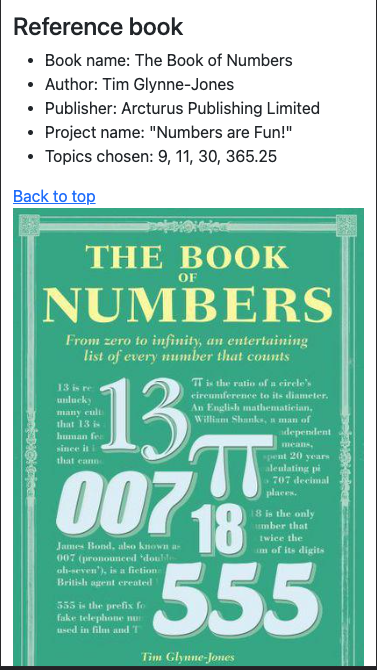
\includegraphics[width=5cm]{images/chn6-grid-xs.png}
\caption{Result of using the grid system on xs screens}
\end{figure}

\begin{figure}[H]
\centering
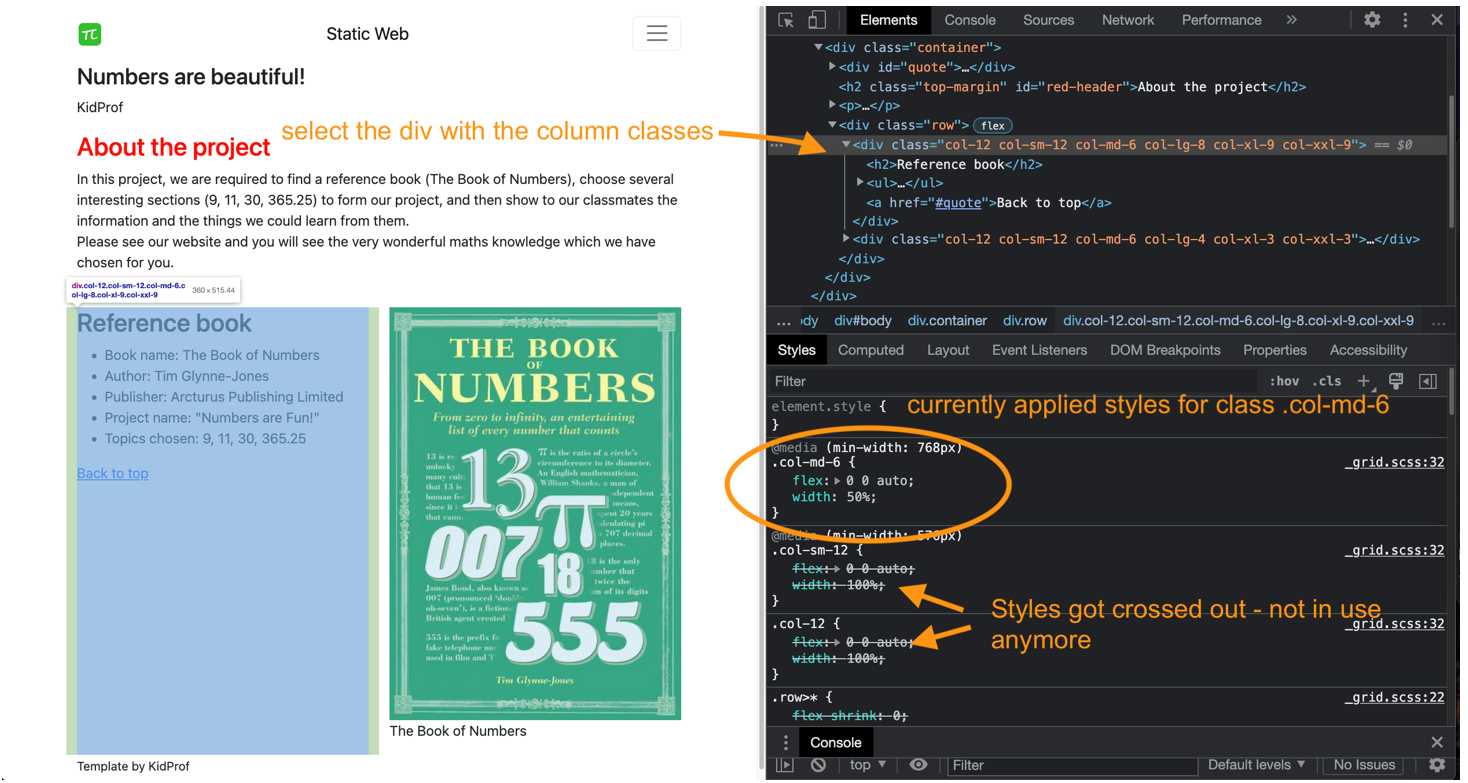
\includegraphics[width=15cm]{images/chn6-grid-md.png}
\caption{Result of using the grid system on md screens, also with illustrations on how to know which screen size we are currently in}
\end{figure}

\begin{figure}[H]
\centering
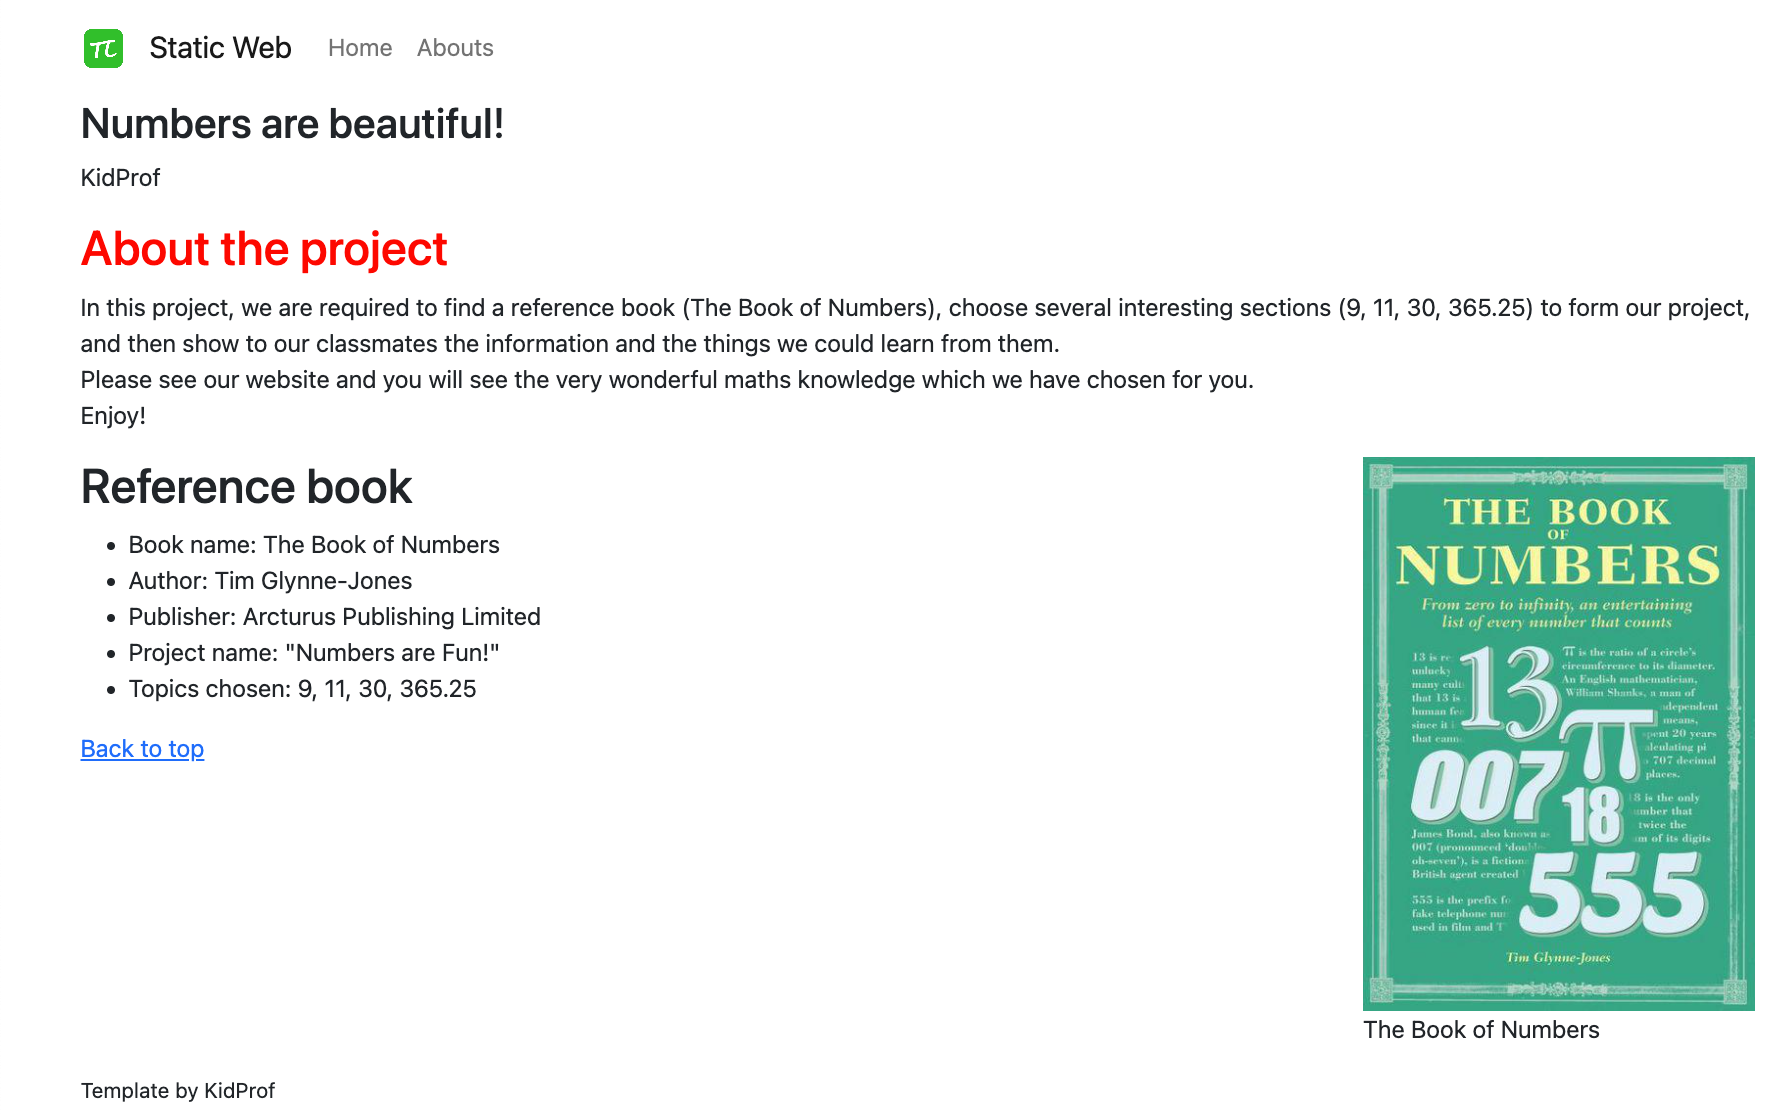
\includegraphics[width=10cm]{images/chn6-grid-xl.png}
\caption{Result of using the grid system on xl screens}
\end{figure}

\subsection{Flexbox}
\label{sec:flexbox}

\textit{Advanced}
\vspace{6mm}

In rare occasions you would like to position an unknown number of elements (like in \cref{sec:navbar}), or a number that is not divisible by 12, then using the grid system might not be a good idea. We can use flexbox in these scenarios. It is \href{https://css-tricks.com/snippets/css/a-guide-to-flexbox/}{well documented}\footnote{Documentation: \url{https://css-tricks.com/snippets/css/a-guide-to-flexbox/}} with clear illustrations, and \href{https://flexboxfroggy.com/}{this URL is an interactive tutorial called Flexbox Froggy (it is very fun)}\footnote{Tutorial: \url{https://flexboxfroggy.com/}}, so I will not repeat it here. In order to use all the styles listed in there, you first have to surround the elements involved with an element with the style \texttt{display: flex;}, bringing all the elements within it to the "flex world".

It could be hard to get right at first, I recommend using the browser developer mode to experiment more with flexbox, add the related stles to different layers of elements and see which ones works, before implementing it in our Less files because we probably cannot get it right first try.

And one side note, learning the concept of flexbox is useful when building apps.

\begin{figure}[h]
\centering
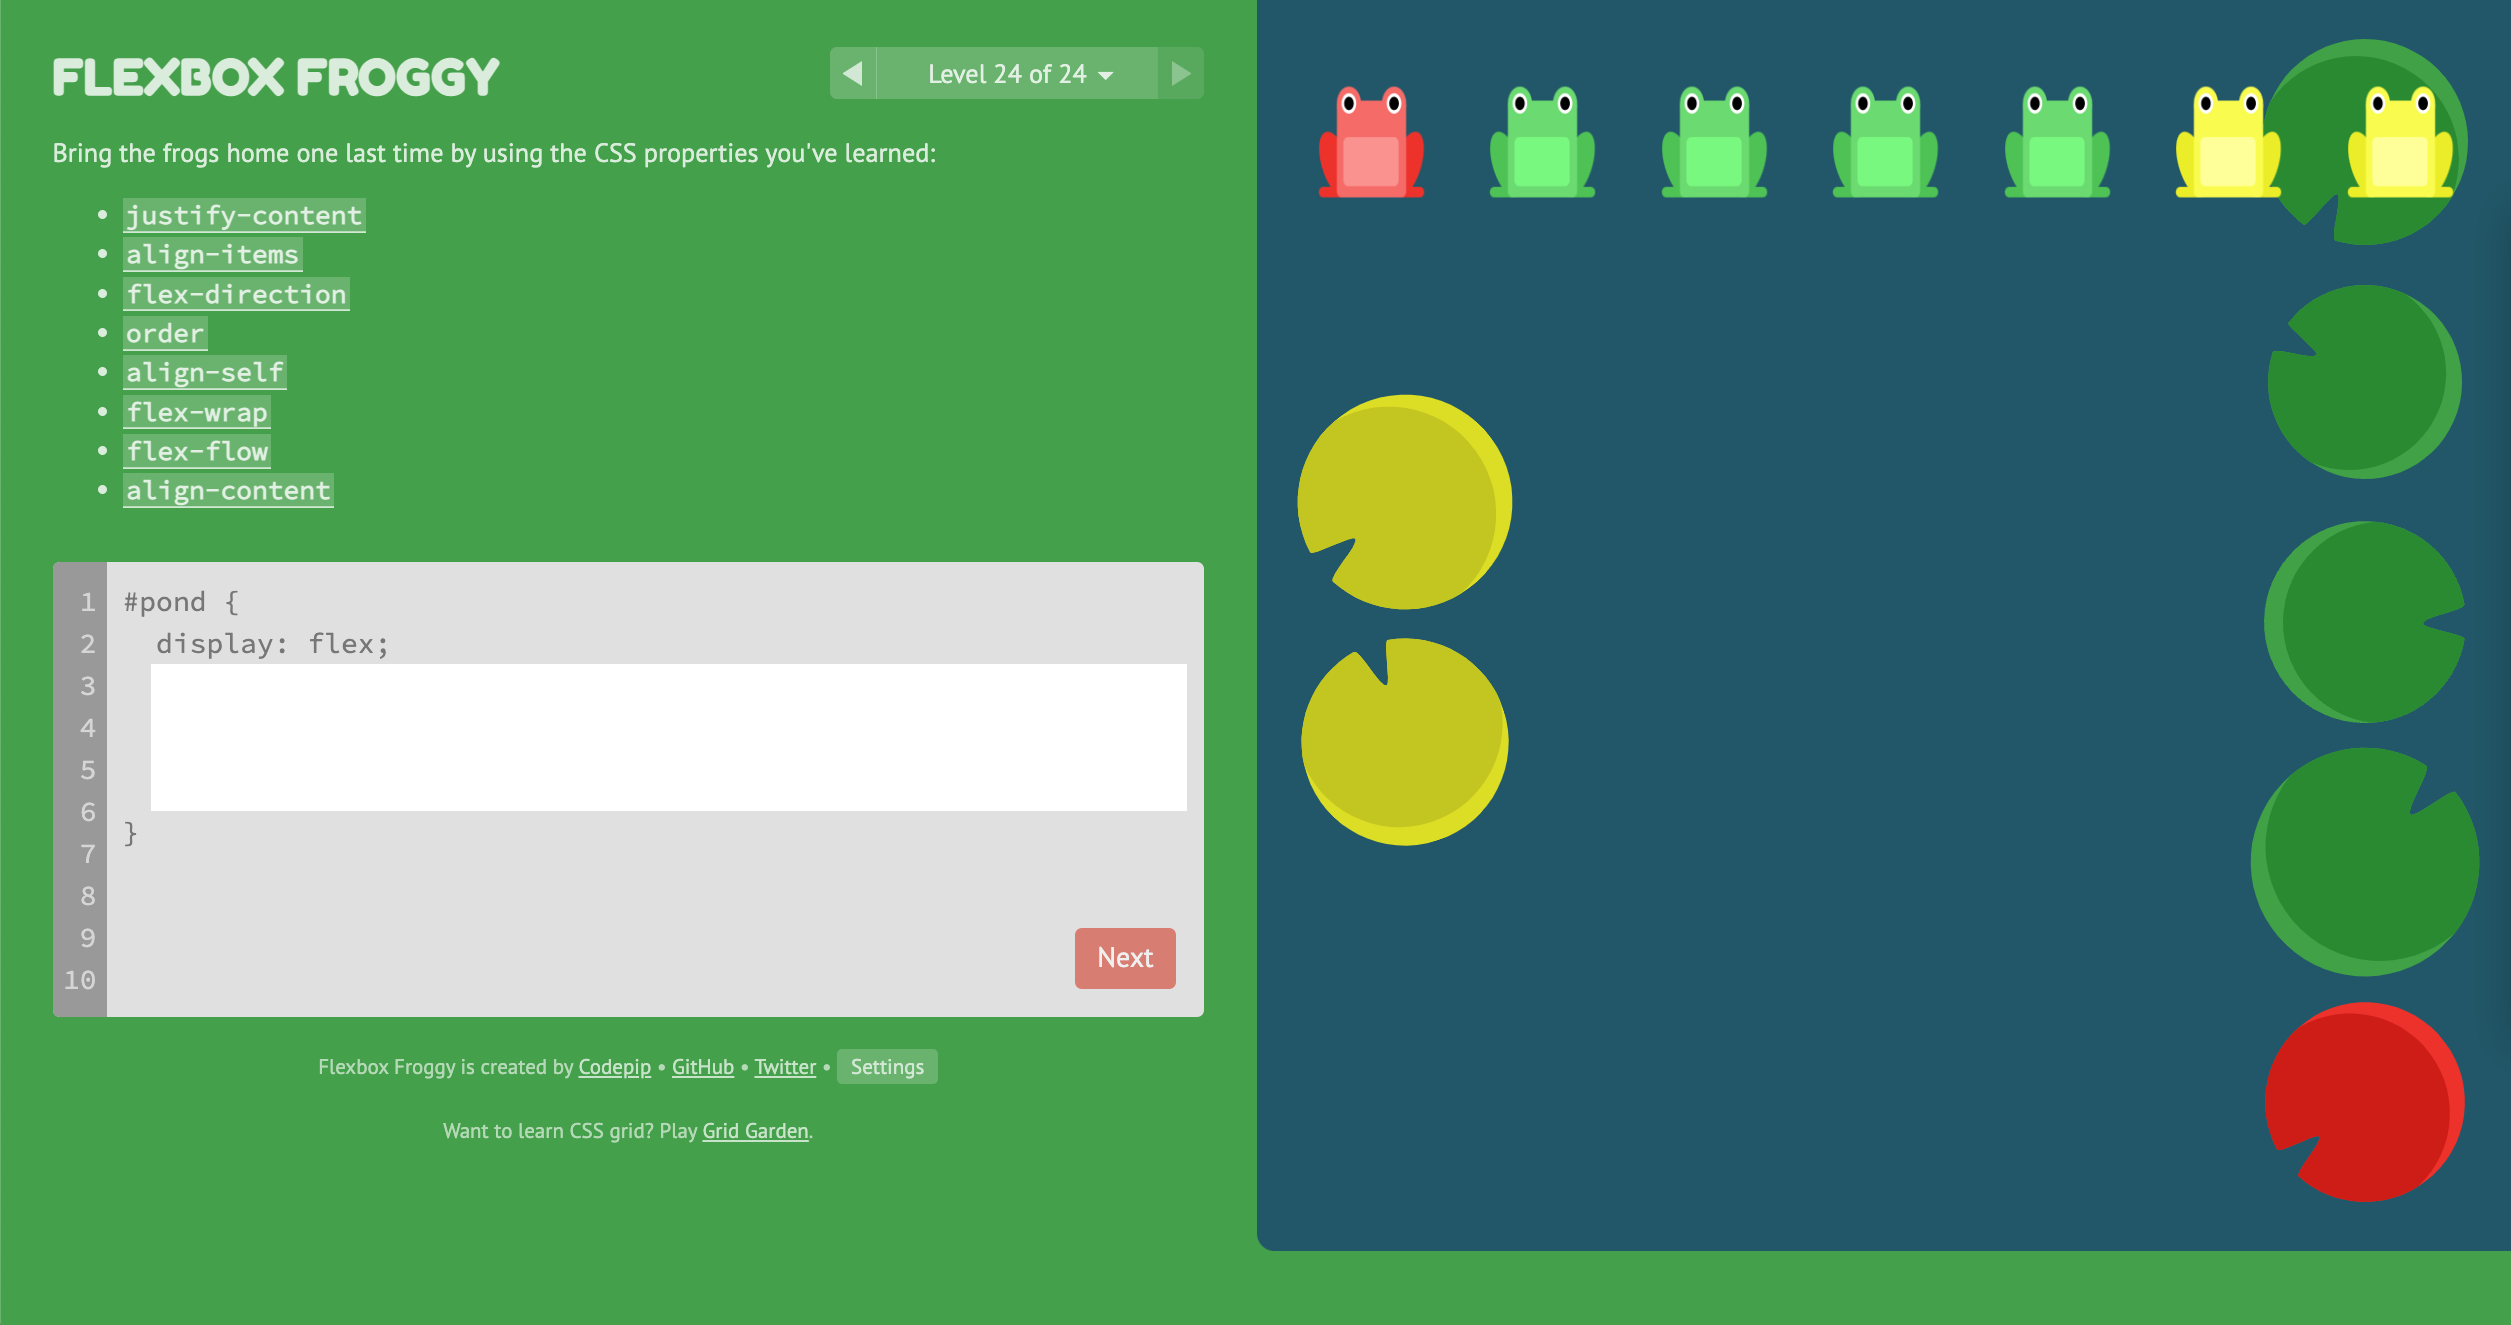
\includegraphics[width=10cm]{images/chn6-flexboxfroggy.png}
\caption{Flexbox Froggy}
\end{figure}

\section{Margins and paddings}
\label{sec:marginpadding}
\label{sec:margin}

\subsection*{Leaving spaces between elements}

Both margins and paddings give spaces between elements, they are the same unless background colour or border is involved, or if the element is clickable.

Say we want to add some space at the bottom of the project description. We can add an ID to the \texttt{p} tag and reference it using that.

\begin{lstlisting}[language=pug]
//- templates/views/abouts.pug
p#proj-desc.
    In this project, ...
\end{lstlisting}

\begin{lstlisting}[language=pug]
// app/styles/site/abouts.less
#proj-desc{
    margin: 0 0 2rem 0;
}
\end{lstlisting}

Note that \texttt{margin} and \texttt{padding} takes 4 arguments, specifying the margin/ padding you want to apply to the \texttt{top}, \texttt{left}, \texttt{bottom}, \texttt{right} of the element. Remember the unit should be \texttt{rem} as explained in \cref{sec:rem}.

Let's try to replace it with a padding.

\begin{lstlisting}[language=pug]
#proj-desc{
    padding: 0 0 2rem 0;
}
\end{lstlisting}

That order is not easy to understand at all. Luckily CSS provides an alternative. You can just specify the direction, separated with a hyphen after \texttt{margin}.

\begin{lstlisting}[language=pug]
#proj-desc{
    margin-bottom: 2rem;
}
\end{lstlisting}

\begin{lstlisting}[language=pug]
#proj-desc{
    padding-bottom: 2rem;
}
\end{lstlisting}

Similarly we got \texttt{margin-left}, \texttt{margin-top}, \texttt{margin-right}, \texttt{padding-left}, \texttt{padding-top}, \texttt{padding-right}. 

We can use both margins and paddings. The resultant spacing would be the sum of spacings. 

\begin{lstlisting}[language=pug]
#proj-desc{
    margin-bottom: 0.5rem;
    padding-bottom: 1.5rem;
}
\end{lstlisting}

The options listed above should be all equivalent. Feel free to change the numbers to get a feel of how large \texttt{rem} is.
\vspace{6mm}

Another cheesy alternative is to add \texttt{br} tags between elements to give the same effect. 

\subsection*{Background colour}

Behaviour of margins and paddings are not the same when you have a background colour. Let's try to add a margin\footnote{It could be simplified as \texttt{margin: 1rem;} but I don't want to confuse you too much.} all around quote where in \cref{sec:nestedstyles} we added a grey background colour for it. Our aim is to move the texts a bit more to the middle because it seems that the texts are too close to the edges of the grey background.

\begin{lstlisting}[language=pug]
#quote{
    ... (add it below your existing styles)
    margin: 1rem 1rem 1rem 1rem;
}
\end{lstlisting}

\begin{figure}[H]
\centering
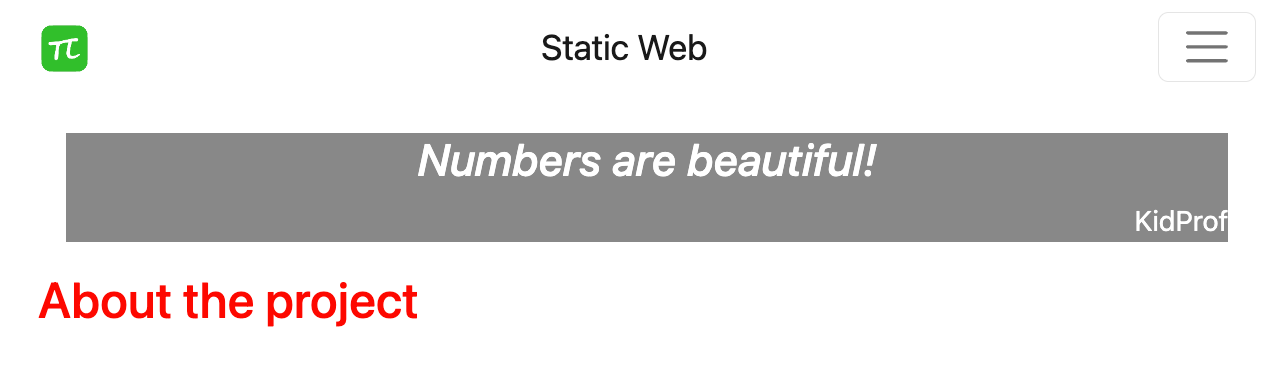
\includegraphics[width=8cm]{images/chn6-quote-margin.png}
\caption{Result of applying margins to the quote}
\end{figure}

Replace it with a padding and notices the differences.

\begin{lstlisting}[language=pug]
#quote{
    padding: 1rem 1rem 1rem 1rem;
}
\end{lstlisting}

\begin{figure}[H]
\centering
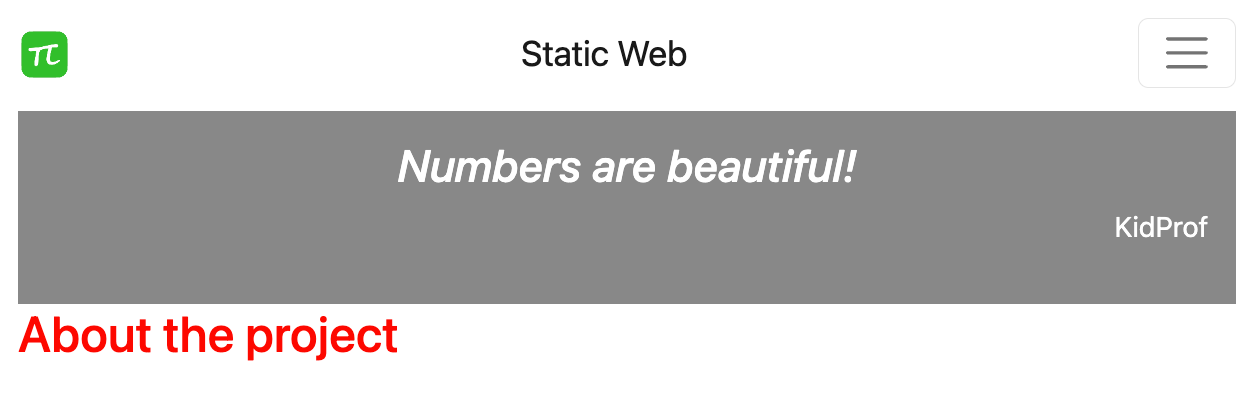
\includegraphics[width=8cm]{images/chn6-quote-padding.png}
\caption{Result of applying paddings to the quote}
\end{figure}

Both the padding and margin pushes the texts inwards for some spacing. Note that padding extends the background colour while margins will not. Seems for our example, adding paddings looks better than adding margins.

Another place where it might be different would be when the element is clickable (e.g. a \texttt{button}), if you click on its padding, it will still respond, but if you click on its margin it will not.
\vspace{6mm}

One side note, I noticed that the quote is quite close to the \texttt{About the project} header, let's add some spacing there as well. Think about whether we should use margin or padding?

\begin{lstlisting}[language=pug]
//- app/styles/site/abouts.less
#quote{
    padding: 1rem 1rem 1rem 1rem;
    margin-bottom: 2rem;
}
\end{lstlisting}

I suppose margin would do a better job here. We want the header to be away from the grey background so we do not want to extend the grey background. 
\vspace{6mm}

Browser developer tools might help a bit, you can scroll to the very bottom of the styles tab, and you can see the margin, border and padding applied to the active element. The active element is also shaded, the blue colour represents the internal contents of the element, the green colour represents its padding and the orange colour represents its margin.

\begin{figure}[h]
\centering
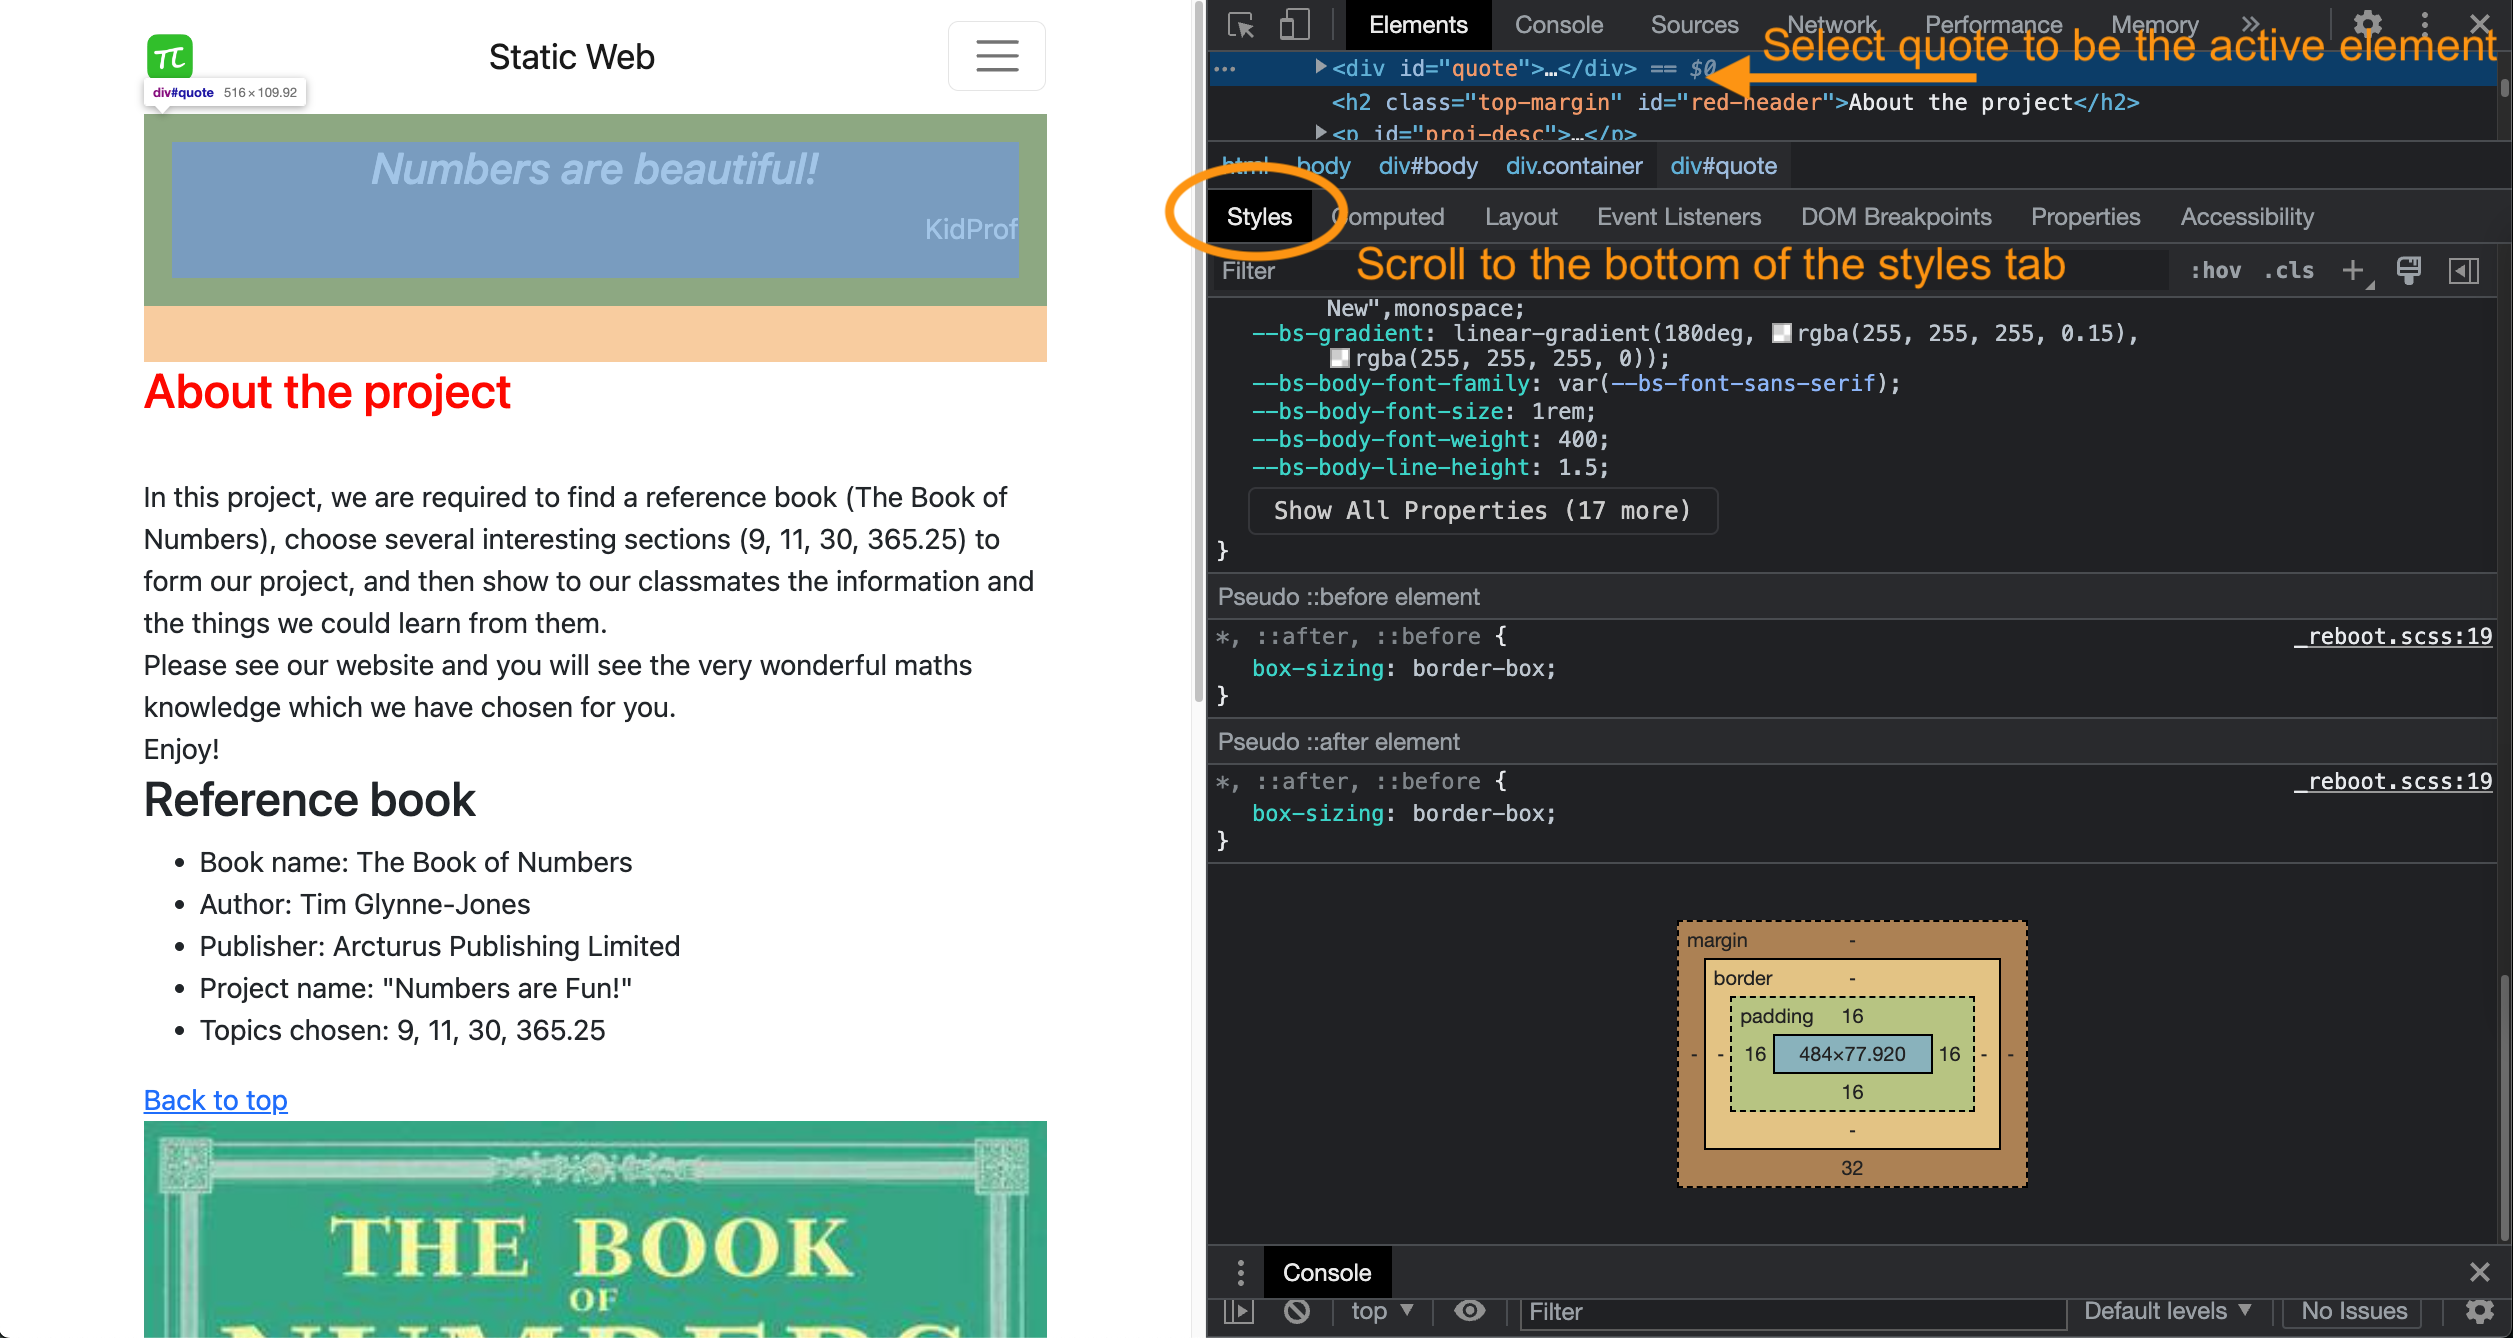
\includegraphics[width=15cm]{images/chn6-quote-chrome.png}
\caption{Browser developer tools that helps with margins and paddings}
\end{figure}

Don't stress yourself out that you need to make it right first try, feel free to experiment around and see which styles makes it look nicer. You could also experiment with the number you put as the attribute. After all styling is an artistic and creative activity. 

\subsection*{Border}

Border will be added between the margin and the padding. \texttt{border} receives 3 arguments - thickness (in \texttt{px}), type (usually \texttt{solid}) and colour. For example, this creates a thin red border around our quote.

\begin{lstlisting}[language=pug]
//- app/styles/site/abouts.less
#quote{
    ... (add it below your existing styles)
    border: 2px solid red;
}
\end{lstlisting}

Ewww. That looks not too great, let's just remove it. The point is to let you have a look on how to add a border. 

\subsection*{Other styling on the quote}

I am just determined to make the quote prettier. So I made the \texttt{h3} tag italic using \texttt{font-style: italic;} and to create rounded edges around the grey background, we uses \texttt{border-radius: 10px;}. 
\vspace{6mm}

How am I sure which property keywords to use? I don't know I just ask Google. (e.g. searching "CSS text italic" and "CSS rounded edges" respectively)
\vspace{6mm}

How am I sure if the numbers are right? (\texttt{10px} for \texttt{border-radius}? \texttt{2rem} for \texttt{margin-bottom}?) I don't know. Just experiment in the browser developer tools until I found it satisfactory.
\vspace{6mm}

To conclude, this is all the styles we applied to the quote.
\begin{lstlisting}[language=pug]
#quote {
    background-color: #888;
    color: white;
    padding: 1rem 1rem 1rem 1rem;
    margin-bottom: 2rem;
    // border: 1px solid red; (commented)
    border-radius: 10px;
    h3{
        text-align: center;
        font-style: italic;
    }
    p{
        text-align: right;
    }
}
\end{lstlisting}

\begin{figure}[H]
\centering
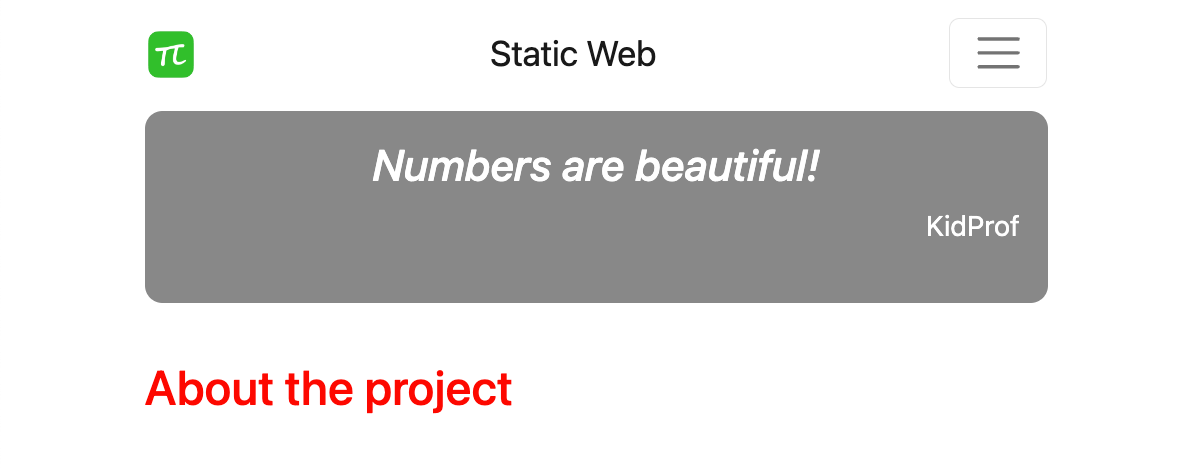
\includegraphics[width=8cm]{images/chn6-quote.png}
\caption{Result of the quote up to \cref{sec:marginpadding}}
\end{figure}


\section{Styling priority}
\label{sec:stylingpriority}

Let's say we add a new style to all \texttt{h3} tags in the whole website, asking them all to be aligned to the right. Remember by convention, we put styles that affect the whole website in \texttt{app/styles/site/layout.less}

\begin{lstlisting}[language=pug]
// recalling what we had in app/styles/site/abouts.less
#quote {
    h3{
        text-align: center;
    }
}
\end{lstlisting}

\begin{lstlisting}[language=pug]
// app/styles/site/layout.less
h3{
    text-align: right;
}
\end{lstlisting}

Notice that it has no effect on the \texttt{h3} tag with text \texttt{Numbers are beautiful!}. Because \texttt{\#quote h3} is more \textbf{specific} than \texttt{h3}. Our original style that tells that particular \texttt{h3} tag to be centred is more specific than the newly defined style which tells all \texttt{h3} tags to be styled. 

How to define more specific systematically? You could follow this URL to get the full answer. But the short answer here (and the answer you need) is that \textbf{styles referencing elements using IDs have priority}.

\begin{figure}[h]
\centering
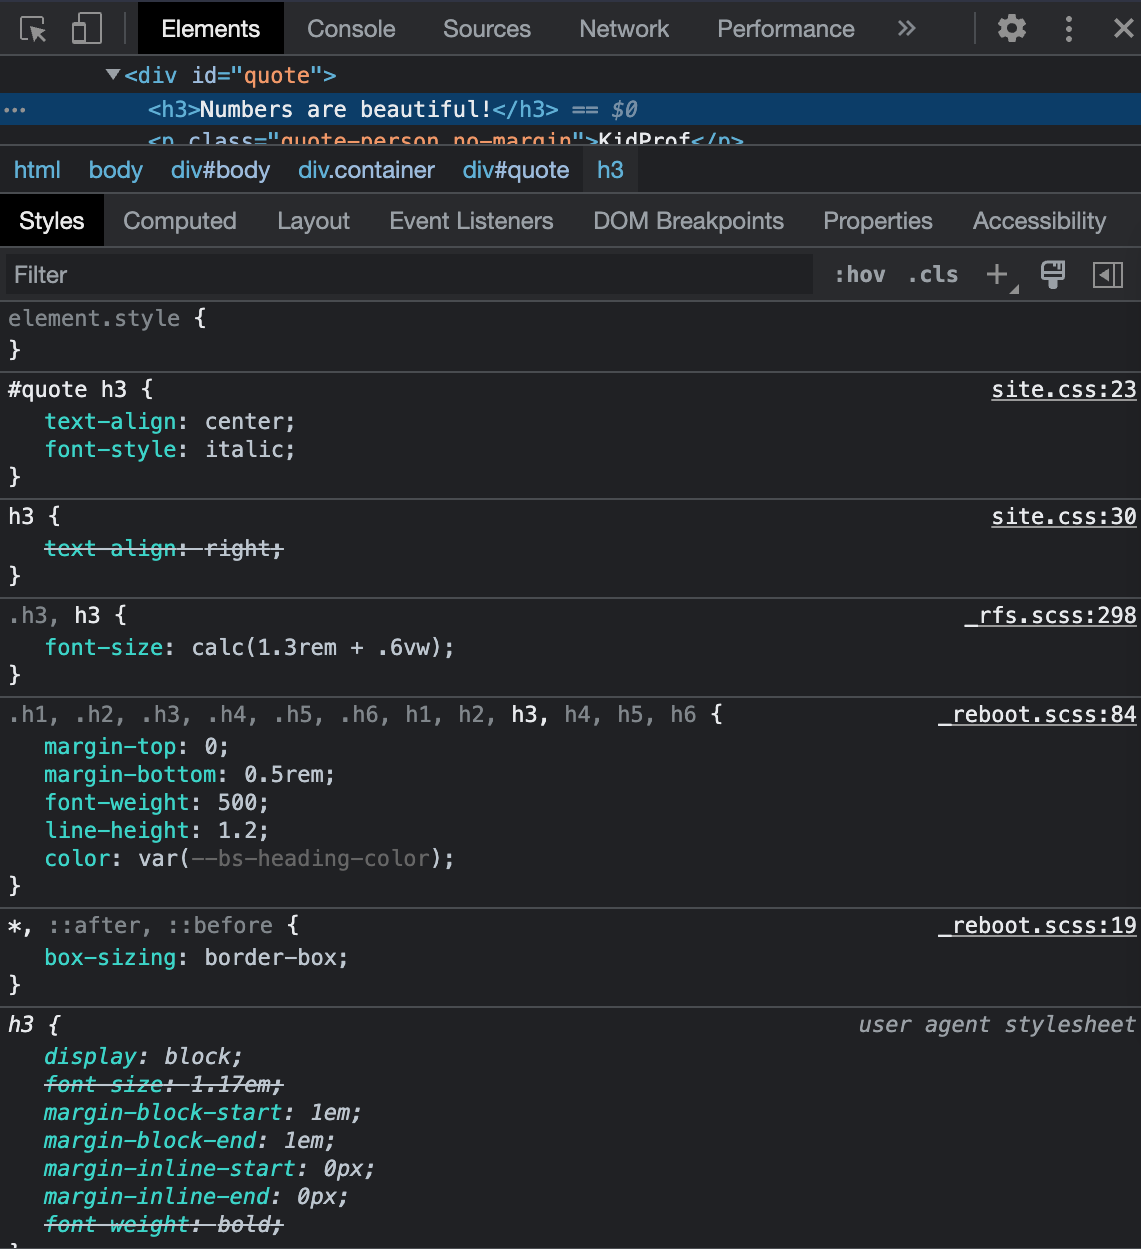
\includegraphics[width=10cm]{images/chn6-stylingpriority.png}
\caption{In the browser developer tools, the style \texttt{text-align: right} is being crossed out, meaning it is being overridden by a more specific style.}
\end{figure}

\subsection*{Prioritising page styles over global styles}

We would usually define some global styles for some web page. However, sometimes we want one or two pages to look different from the rest of the pages. We may end up with conflicting styles like what we had previously, and the priority is not clear. Remember just writing your code in \texttt{abouts.less} would not help you increase the priority of your styles, doing so is just a convention.  

However, we can do something to enforce the convention. We can add an ID surrounding all elements in the abouts page.

\begin{lstlisting}[language=pug]
//- app/templates/views/abouts.pug
extends ../layouts/default

block content
    #abouts //- <-- ID here
        .container 
    	#quote
    		....
    	h2#red-header.top-margin About the project
    	p#proj-desc.
    		...
    	.row
                ...
\end{lstlisting}

We also enclose all styles for the abouts page with an ID.

\begin{lstlisting}[language=pug]
//- app/styles/site/abouts.less
#abouts{
    #bookofnumbers{
        width: 100%;
    }
    .larger-text{
        font-size: 1.25rem;
    }
    ...
}
\end{lstlisting}

Now all code inside \texttt{abouts.less} only applies to the abouts page but not the other pages, and also because of the ID, our code has higher priority than the global styles we defined in \texttt{layouts.less}

As an example, we are going to add a background colour to the pages. By default, I want all pages to have a light blue colour (colour code: \texttt{\#BAE9FF}), however, I want the abouts page to have a yellow colour (color code: \texttt{\#F9F0BB}).

We can achieve that by:

\begin{lstlisting}[language=pug]
// app/styles/site/layout.less - styles for all pages
body{ //styling the whole HTML body
    background-color: #BAE9FF;
}
\end{lstlisting}

\begin{lstlisting}[language=pug]
// app/styles/site/abouts.less - styles for the abouts page
#abouts {
    background-color: #F9F0BB;
}
\end{lstlisting}

\cref{fig:aboutsfinal} gives the result of the styles. Might not be what you expected, because the navbar and the footer are still using the default global light blue colour. Sadly we could not do any better because currently the \texttt{\#abouts} ID is only controlling the things under the \texttt{block content} (see \cref{sec:puglayouts}). Unfortunately it has to stay like that for a while until \cref{sec:navbar}, where we move up the ID to \texttt{layouts.pug} with the help of Pug variables.

\section{Using variables in Less}
\label{sec:lessvariables}
There are two important Less features that CSS doesn't have.
\begin{itemize}
\item Nested styles in the form of multiple curly braces.

\begin{lstlisting}[language=pug]
// LESS
#abouts {
    #bookofnumbers { ... }
    .larger-text { ... }
    #quote {
        h3 { ... }
        p { ... }
    }
}
\end{lstlisting}

\begin{lstlisting}[language=pug]
// CSS 
#abouts #bookofnumbers { ... }
#abouts .larger-text { ... }
#abouts #quote h3 { ... }
#abouts #quote p { ... }
\end{lstlisting}

Less can certainly allow you write \textit{less} code.

\item Variables, which we would discuss now

Variable names must start with an @. You are advised to put all variables in \texttt{app/styles/site/variables.less} We define new variables like this:

\begin{lstlisting}[language=pug]
//- app/styles/site/variables.less
@home-bg-color: #BAE9FF;
@abouts-bg-color: #F9F0BB;
\end{lstlisting}

We use variables like this:

\begin{lstlisting}[language=pug]
// app/styles/site/layout.less
body{
    background-color: @home-bg-color;
}
\end{lstlisting}

\begin{lstlisting}[language=pug]
// app/styles/site/abouts.less
#abouts {
    background-color: @abouts-bg-color;
}
\end{lstlisting}

These changes should not affect the look of the page at all. 

Less can certainly allow you remember \textit{less} things.

\end{itemize}

We would end our work on styling the sample abouts page for the time being. Here is the final code and the final web page for now.

\begin{lstlisting}[language=pug]
// app/styles/site/abouts.less
#abouts{
    background-color: @abouts-bg-color;
    #bookofnumbers{
        width: 100%;
    }
    
    .larger-text{
        font-size: 1.25rem;
    }
    
    #red-header{
        color: red;
    }
    
    #proj-desc{
        margin: 2rem 0 0 0;
    }
    
    // .no-margin{
    //     margin-bottom: 0;
    // }
    
    #quote {
        background-color: #888;
        color: white;
        padding: 1rem 1rem 1rem 1rem;
        margin-bottom: 2rem;
        // border: 1px solid red;
        border-radius: 10px;
        h3{
            text-align: center;
            font-style: italic;
        }
        
        p{
            text-align: right;
        }
    }
}
\end{lstlisting}

\begin{figure}[h]
\centering
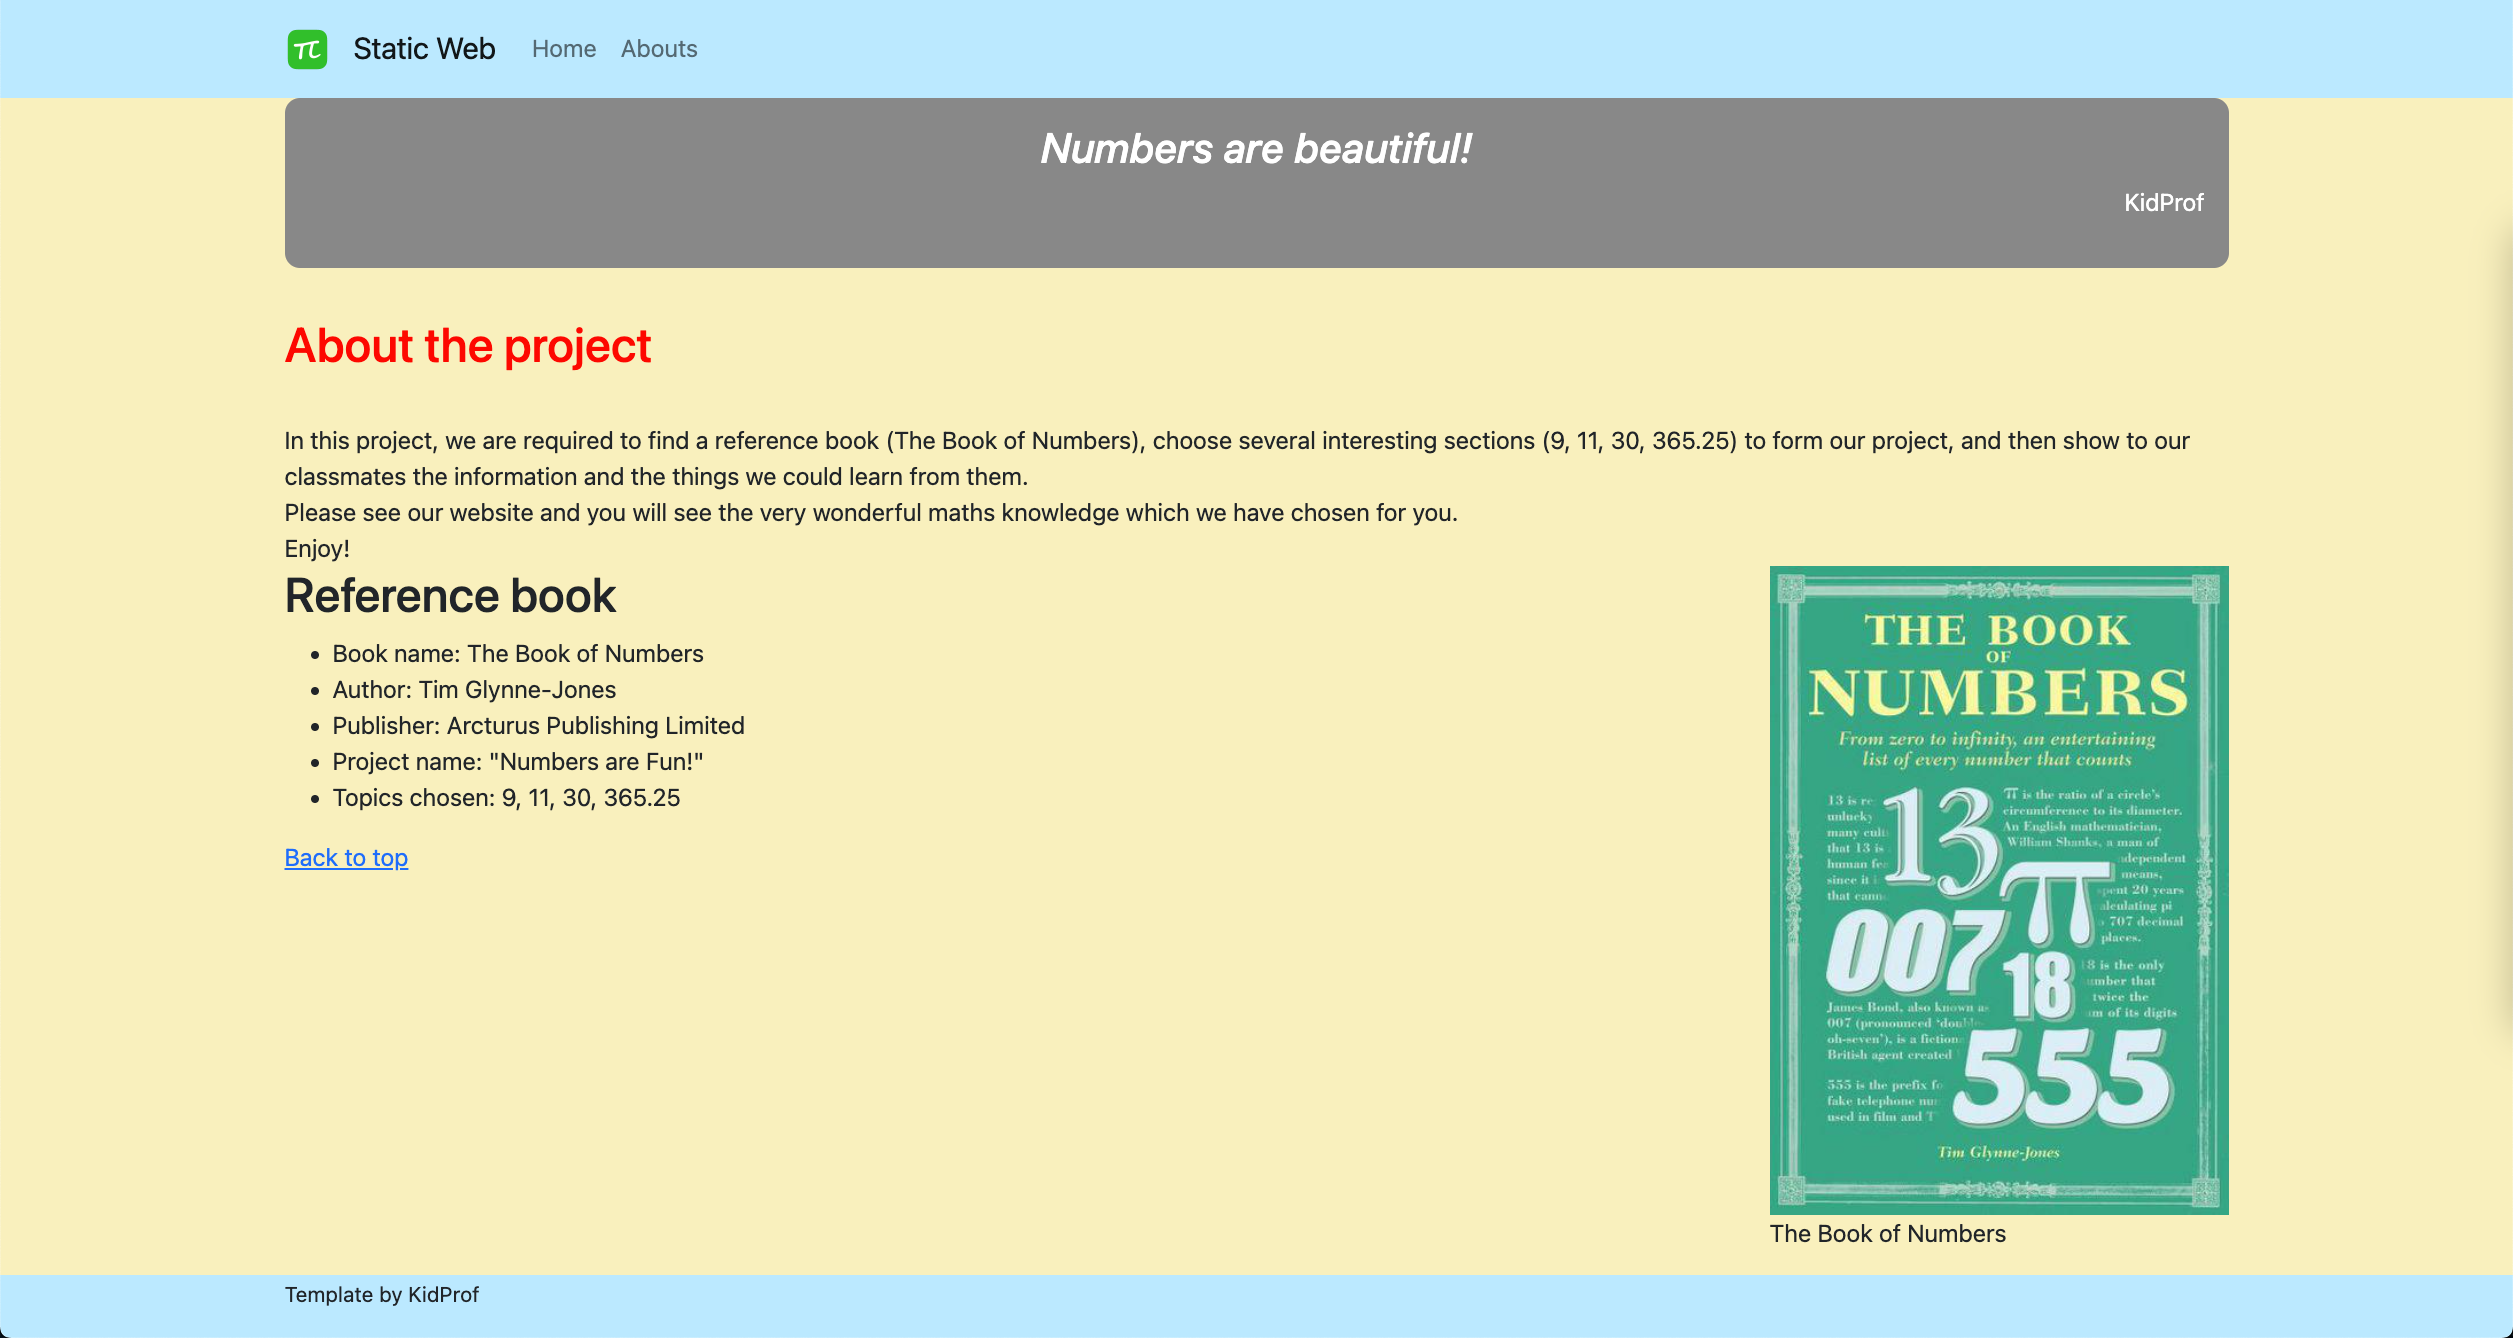
\includegraphics[width=13cm]{images/chn6-background-colour.png}
\caption{Our progress on the abouts page up till \cref{sec:lessvariables}}
\label{fig:aboutsfinal}
\end{figure}